\chapter{Linear metric labelling problem}

In this chapter, we will present one of the major results in this thesis, the $L(p_1,p_2,p_3)$-labelling of complete $m$-ray trees. Since there are only three parameters in this labelling system, from this time onwards we will call it $\lhpq$-labelling, unless we refer to a labelling system with infinitely many parameters. In the first section, we will give definitions and notation. We will then present a review of some know results. In Section 3.3, we present our results of $L(h,1,1)$-labelling of complete $m$-ary trees. Section 3.4 extend the $L(h,1,1)$-labelling result of complete $m$-ary trees to the general case; i.e., the $\lhpq$-labelling of complete $m$-ary trees. In the last section, we move onto the $\lhpq$-labelling of a broader class of trees that contain the set of complete $m$-ary trees as a subset. 



\section{Definitions and notation}

A linear metric $\lhpq$-labelling of a graph $G$ is an assignment of vertices of $G$ to non-negative integers such that vertices at distance $1$, $2$ or $3$ apart are mapped to integers with difference at least $h, p$ or $q$. Precisely, we have the following definition: 
\begin{definition}
A graph $G$ is said to be $\lhpq$-labelled if there is a map  
\[
f : V(G) \rightarrow \{0, 1, 2, \dots\}, 
\]
which respects the following constraints: 
\begin{itemize}
\item $|f(u) - f(v)| \ge h$, if $uv \in E(T)$;
\item $|f(u) -f(v)| \ge p$, if $d(u,v) = 2$;
\item $|f(u) - f(v)| \ge q$, if $d(u,v)=3$,
\end{itemize}
where $h\ge p \ge q \ge 1$ are integers. 
\end{definition}

According to this definition, it is noticed that there exists a maximum and a minimum label. Therefore, we define the \textit{span} of an $\lhpq$-labelling of a graph $G$ to be the difference between these maximum and minimum label for vertices of $G$. We use $span(f)$ to denote this concept. Furthermore, the {\it{minimum span}} of the labelling $f$ on the graph $G$ is defined as the smallest span over all $\lhpq$-labellings of $G$. The standard notation for the minimum span of an $\lhpq$-labelling of a graph $G$ is $\lamhpq(G)$.

\begin{remark}
\label{0}
Since the above function $f$ assigns non-negative integers to vertices of a graph $G$, it is convenient to always set the minimum label to be $0$. In this case, the span of $f$ is just the maximum label used by $f$, and the minimum span is the smallest maximum label assigned to vertices of $G$ by some $\lhpq$-labellings. 
\end{remark}

Let us go through an example of an $L(h,1,1)$-labelling of a complete $m$-ary tree. 

\begin{example}
Let $T_{2,2}$ be a complete $m$-ary tree with height $2$. Consider two different $L(2,1,1)$-labellings,  $f_1$ and $f_2$ on $T_{2,2}$ as shown in Fig. \ref{linear metric labelling} (a) and (b) respectively.

According to the above definitions, we have $span(f_1) = 7$ and $span(f_2) = 5$. In fact, it will be proved in Section 3.3 that the minimum span of $L(2,1,1)$-labelling of $T_{2,2}$ equals $span(f_2)$; i.e., $\lambda_{2,1,1}(T) = span(f_2) = 5$. 
  

\begin{figure}
\centering
      \vspace{-10pt}
    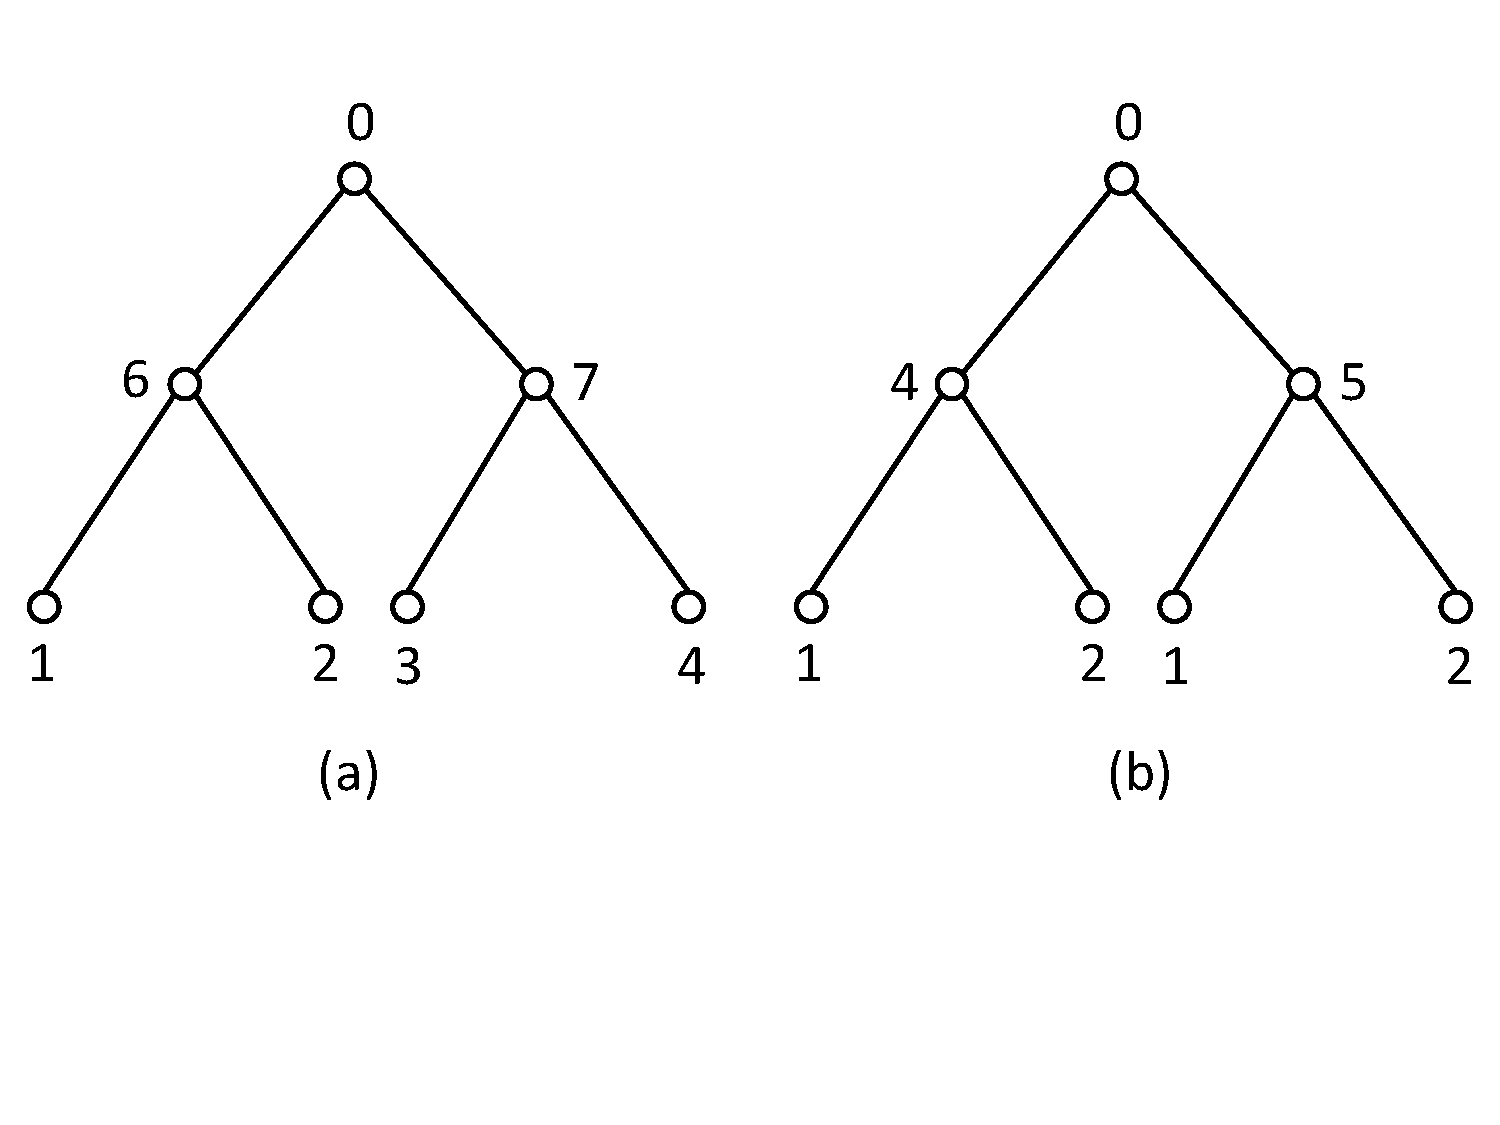
\includegraphics[scale=0.4]{../figures/fig3-1.pdf}
        \vspace{-50pt}
\caption{Two $L(h,1,1)$-labellings of $T_{2,2}$}
\label{linear metric labelling}
\end{figure}

\end{example}




%%%%%%%%%%%%%%%%%%%%%%%%%
\section{Known results for linear metric labelling problems}

In this section, we give the reader some ideas of what have been done in this area. It will include many linear metric labelling results for different types of graphs. Just remind the reader that we use $\Delta$ to denote the maximum degree of a graph. 

%For distance two constraints linear metric $L(p_1, p_2)$-labelling, when $p_1=p_2=1$ it is what we normally called graph clolouring. In this case, the minimum span is just the chromatic number for graph colouring. In the following, we will give some $L(1,1)$-labelling results of graphs. 

\subsection{Paths and cycles}

One of the earliest graph labelling problems is the $L(2,1)$-labelling of graphs, which was studied by \cite{yeh90} in his Ph.D thesis. Yeh first presented $L(2,1)$-labelling results of an $n$ vertices path $P_n$. He proved that the minimum span
\begin{align*}
\lambda_{2,1}(P_n) = 
\begin{cases}
2 & \text{ if } n = 2,\\
3 & \text{ if } n = 3 \text{ and }4,\\
4 & \text{ if } n \ge 5.
\end{cases}
\end{align*}
Based on this result, \cite{griggs92} proved that $\lambda_{2,1}(C_n) = 4$, for any $n$-cycle $C^n$. Later on, \cite{georges95} solved an even general problem. They proved that for $p_1 \ge p_2 \ge 1$, the minimum span of the $L(p_1, p_2)$-labelling of $P_n$ is 
\begin{align*}
\lambda_{p_1, p_2}(P_n) = 
\begin{cases}
0 & \text{ if } n =1, \\
p_1 & \text{ if } n = 2, \\
p_1 + p_2 & \text{ if } n = 3 \text{ or } 4, \\
p_1 + 2p_2 & \text{ if } n \ge 5 \text{ and } p_1 \ge 2p_2, \\
2p_1 & \text{ if } n \ge 5 \text{ and } p_1 \le 2p_2. 
\end{cases}
\end{align*}
If $p_1 \ge p_2 \ge 1$ and $p_1/p_2 > 2$, then the minimum span of the $L(p_1, p_2)$-labelling of $C^n$ is 
\begin{align*}
\lambda_{p_1, p_2}(C_n) = 
\begin{cases}
2p_1 & \text{ if } n \ge 3 \text{ is odd}, \\
p_1+2p_2 & \text{ if } n \equiv 0 \pmod{4}, \\
2p_1 & \text{ if } n \equiv 2 \pmod{4} \text{ and } p_1/p_2 \le 3,\\
p_1+3p_2 & \text{ if } n \equiv 2 \pmod{4} \text{ and } p_1/p_2 >3,
\end{cases}
\end{align*} 
If $p_1 \ge p_2 \ge 1$ and $p_1/p_2 \le 2$, then 
\begin{align*}
\lambda_{p_1, p_2}(C_n) = 
\begin{cases}
2p_1 & \text{ if } n \equiv 0 \pmod{3}, \\
4p_2 & \text{ if } n = 5, \\
p_1 + 2p_2 & \text{ otherwise.} 
\end{cases}
\end{align*}

%%%%%%%%%%%%%%%%%%%%%%%%%%%%%%%%%%%%%%%
\subsection{Trees}

\citet{griggs92} in the same paper also proved that the minimum span of the $L(2,1)$-labelling of any tree $T$ with maximum degree $\Delta \ge 1$ is $\Delta+1$ or $\Delta+2$. \cite{chang00} generalised Griggs and Yeh's studies to the $L(h,1)$-labelling problem and proved that the minimum span $\Delta+d-1 \le \lambda_{h, 1}(T) \le \min\{\Delta+2d-2, 2\Delta+d-2\}$, where both the lower and upper bounds are attainable. 

For distance three constraint linear metric labelling problem  of trees, there are also many well-known results. One of the most significant results proved by \cite{zhou10} is the $L(h,1,1)$-labelling problem for trees. The authors proved that the minimum span of the $L(h,1,1)$-labelling of any finite tree $T$ with diameter at least $3$ or an infinite tree with finite maximum degree is bounded as follows: 
\begin{align*}
&\max \left\{\max_{uv \in E(T)} \min \{d(u), d(v)\} +h-1, \Delta_2(T) -1\right\} \\
&\le \lambda_{h,1,1}(T) \le \Delta_2(T) +h-1 
\end{align*}
where $\Delta_2(T) := \max_{uv \in E(G)} (d(u) + d(v))$. Such an edge $uv \in E(T)$ is called an \emph{heavy edge}.  

Furthermore, define $\delta^*(T) := \min_{u \in V(T), d(u) \ge 2} d(u)$. \citeauthor{zhou10} proved that if $h \le \delta^*(T)$, then the upper bound can be decreased by $1$; i.e., $\lambda_{h,1,1}(T) \le \Delta_2(T) +h-2$. They also proved that for some special trees such as the caterpillar, both the lower bound and the improved upper bound are attainable. 


 
 
%%%%%%%%%%%%%%%%%%%%%%%%%%%%%%%%%%%%%%%%%%%%%%%%

\subsection{Planar graphs}
If a graph can be drawn on a plane without edge crossing, then we say such a graph is a \emph{planar graph}. 

For the $L(1,1)$-labelling of planar graphs, \cite{wegner97} conjectured
\begin{align*}
\lambda_{1,1}(G) = \chi(G) \le 
\begin{cases}
(3/2\Delta) + 1 & \text{ if } \Delta \ge 8, \\
\Delta+4 & \text{ if } 4 \le \Delta \le 7, \\
7 & \text{ if } \Delta = 3.
\end{cases} 
\end{align*}
Moreover, he conjectured that for $\Delta = 3$, the upper bound can be reduced to $6$. These two conjectures are still open for now. 

Recently, many people proved upper bounds for the chromatic number $\chi(G)$ of planar graphs $G$. Among all these results, the most impressive one is published by \cite{molloy05}. They proved that $\lambda_{1,1}(G) \le \lceil \frac{5}{3}\Delta \rceil + 77$ for any planar graph $G$. In particular, if $G$ has maximum degree $\Delta \ge 241$ then $\lambda_{1,1}(G) \le \lceil \frac{5}{3}\Delta \rceil + 24$. 

For $L(2,1)$-labelling of planar graphs $G$, \cite{jonas93} proved that $\lambda_{2,1}(G) \le 8\Delta - 13$. This bound was improved by \cite{van03} when solving the $L(p_1,p_2)$-labelling problem of planar graphs. They proved that the minimum span for any planar graph $G$ is bounded by $\lambda_{p_1,p_2}(G) \le (4p_2-2)\Delta + 10p_1+38p_2-23$, where $p_1 \ge p_2 > 0$. Later on, this upper bound is further improved to $p_2\lceil \frac{5}{3} \Delta \rceil + 18p_1+77p_2-18$ by \cite{molloy05}.

%%%%%%%%%%%%%%%%%%%%%%%%%%%%%%%%%%%%%%%%%%%%%%%%

\subsection{Outerplanar graphs} 
\label{linear outerplanar}
We say a graph is \emph{outerplanar} if drawing all its vertices on a path and its edges on one side of the path will not cause any edge crossing. Alternatively, an outerplanar graph is a graph such that when connecting an extra vertex to all its vertices does not cause any edge crossing. An outerplanar graph is planar, but the converse is not always true. 

\textbf{$L(1,1)$-labelling}. \cite{agnarsson04} proved an optimal upper bound for outerplanar graphs with smaller maximum degree $\Delta$. Precisely, for any outerplanar graph $G$, the minimum span is $\lambda_{1,1}(G) \le \Delta+2$ if $\Delta=2$ and $\lambda_{1,1}(G) \le \Delta+1$ if $\Delta=3,4$ and $6$. 
\\
\\
\textbf{$L(2,1)$-labelling.} \cite{jonas93} in his paper also proved an upper bound for the minimum span of the $L(2,1)$-labelling of outerplanar graphs $G$; i.e., $\lambda_{2,1}(G) \le 2\Delta+2$. Based on this result, \cite{bodlaender04} in their paper improved this upper bound to $\Delta+8$. More importantly, they conjectured that the bound can be improved to $\Delta+2$. Motivated by this, \cite{calamoneri04} proved the conjecture to be true for $\Delta \ge 8$ but false for $\Delta=3$. They also proved that $\lambda_{2,1}(G) \le \Delta+5$ for any outerplanar graph $G$ with $\Delta=3$. \cite{zhou11} recently improved \citeauthor{calamoneri04}'s upper bound to $\lambda_{2,1}(G) \le \Delta+3$ for every outerplanar graph $G$ with maximum degree $\Delta=3$. They mentioned in the paper that this bound is attainable by infinitely many outerplanar graphs. 
\\
\\
\textbf{$L(h,1,1)$-labelling.} For distance three constraint linear metric labelling of outerplanar graphs, \cite{calamoneri07} proved that $3\Delta-3 \le \lambda_{1,1,1}(G) \le  4\Delta-2$. In particular, the upper bound can be improved to $3\Delta+9$ if $G$ has maximum degree $\Delta \ge 6$. As a general result, they proved that $\lambda_{h,1,1}(G) \le 3\Delta+2h+7$ for $\Delta \ge h+5$. 

So far, we introduced to the readers many well-known results in this ares. In the following, we will present our own results. 



%%%%%%%%%%%%%%%%%%%%%%%%%%%%%%%%%%%%%%%%%%%%%%%%






%%%%%%%%%%%%%%%%%%%%%%%
\section{The $L(h,1,1)$-labelling of complete $m$-ary trees}
Let  $u_0 \in V(\tmk)$ be the root of $\tmk$, $u_i \in V(\tmk)$ be the vertex that is distance $1$ to $u_0$; $u_{ij} \in V(\tmk)$ be the vertex that is distance $2$ to $u_0$. In general, 
%First, let us define some new notations for complete $m$-ary trees that. Note that these notations are not standard, they are just for the convenience of proofs regarding to complete $m$-ary trees. We define the following: 
%\begin{itemize}
%\item $\VV_i := \{u \in V(\tmk) \mid d(u, u_0) = i\}$, where $i \in [1,m]$
%\item $C(u) :=$ children of a vertex $u \in V(\tmk)$
%\item $P(u) :=$ parent of a vertex $u \in V(\tmk)$
$u_{\underbrace{ij\dots k}_\text{n}} \in V(\tmk)$ is the vertex that is distance $n$ to the root $u_0$, for $i, j, \dots, k \in [1, m]$. \footnote{Define $[1,m]:=\{1, 2, 3, \dots, m-1, m\}$.} 
%\end{itemize}


\begin{lemma}
\label{reuse}
Suppose $f$ is an $L(h,1,1)$-labelling of a complete $m$-ary tree $\tm2$. Then it is possible to assign same labels to $C(u_i)$ and $C(u_j)$ for $i \neq j$ without causing conflict,\footnote{By causing conflict we mean the map $f$ violates the $L(h,1,1)$-labelling conditions.} that is, 
\[
f(C(u_i)) = f(C(u_j)), \text{ for } i \neq j. 
\]
\end{lemma}

\begin{proof}
Without loss of generality, let us consider the sets $C(u_1)$ and $C(u_2)$. We know that $u_{1j} \in C(u_1)$ and $u_{2j} \in C(u_2)$, then for all $j \in [1,m]$ it follows that 
\begin{align}
\label{dis4}
d(u_{1j}, u_{2j}) = 4.
\end{align}
By conditions of $L(h,1,1)$-labelling, $u_{1j}$ and $u_{2j}$ can receive the same label. Thus in general, $C(u_i)$ and $C(u_j)$ can be labelled by the same labels.  
\end{proof}
\qed

\begin{lemma}
\label{lem:consh11} Let $f$ be an $L(h,1,1)$-labelling of a complete $m$-ary tree $\tm2$. Suppose $f$ labels $\tm2$ in the following way: 
\begin{enumerate}[(1)]
\item $f(N(u_1))$ and $f(C(u_0))$ are consecutive label sets for vertices of $\tm2$;
\item $\min \{f(N(u_1))\} - \max\{f(C(u_0))\} = h$ or $\min\{f(C(u_0))\} - \max\{f(N(u_1))\} = h$.
\end{enumerate}
Then, for any other $L(h,1,1)$-labelling of $\tm2$, say $g$, we have 
\begin{align}
\label{minimum}
span(f) \le span(g). 
\end{align}
More importantly, the span of $f$ achieves an exact value, that is, 
\begin{align}
\label{exact} 
span(f)= 2m+h-1. 
\end{align}
\end{lemma}

Note that according to Lemma \ref{reuse}, here we only deal with $f(N(u_1))$ as $f(C(u_i)) = f(C(u_j))$ for $i \neq j$.
\\
\begin{proof}
The proof of this lemma refers to the proof of Lemma \ref{lem:conshpq}, which is a generalised version of this lemma. 
\end{proof}
\qed
\\
%As a bound for the minimum span of $L(h,1,1)$-labelling on trees is given by Theorem \ref{thm:deb} (Refer to Theorem $1$ in {deborah}), we can start with applying this theorem to the family of complete $m$-ary trees. If possible, improve the bound from then. 

%Notice that for a complete $m$-ary tree $T$, the $\Delta_2$ value varies for different height of $T$. In particular, $\Delta_2(T) = 2m+1$ for height $k=2$ and $\Delta_2(T) = 2m+2$ for height $k \ge 3$. By Theorem \ref{thm:deb}, we have 

%\begin{align*}
%\max\{m+h-1, 2m\} &\le \l \le 2m+h, \text{ when } k = 2 \\
%\max\{m+h, 2m+1\} &\le \l \le 2m+h+1, \text{ when } k \ge 3
%\end{align*}

%By definition of $\delta^*(T)$ \cite{zhou00}, for a complete $m$-ary trees $T$ we have $\delta^*(T) = m$. Assume $h \le m =  \d$, we have $2m > m+h-1$ and $2m+1 > m+h$. By improvement of the upper bound in \cite{zhou00}, the upper bounds above can also be improved. Thus we have 

%\begin{align}
%2m &\le \lambda_{h,1,1}(T) \le 2m+h-1, \text{ when } k = 2 \text{ and } h \le m \\
%\label{kge3hlem}
%2m+1 &\le \lambda_{h,1,1}(T) \le 2m+h, \text{ when } k \ge 3 \text{ and } h \le m
%\end{align}

%Assume $h > m$, then results in \cite{zhou00} do not reduce the upper bound. Hence we have 
%\begin{align}
%m+h-1 &\le \l \le 2m+h, \text{ when } k = 2 \text{ and }h > m \\
%\label{kge3hgm}
%m+h &\le \l \le 2m+h+1, \text{ when } k \ge 3 \text{ and } h > m
%\end{align}
The following is our major result for the minimum span of $L(h,1,1)$-labelling problems on the family of complete $m$-ary trees. 

\begin{theorem}
\label{thm:h11} 
For a complete $m$-ary tree $\tmk$, the minimum span of $L(h,1,1)$-labelling of $\tmk$ is
\begin{align}
\label{h11}
 \lambda_{h,1,1}(\tmk) =
  \begin{cases}
   2m+h-1 & \text{for } k = 2, \\
   2m+h       & \text{for } k \ge 3.
  \end{cases}
\end{align}
\end{theorem}

To prove this theorem, let us see the following lemma first. 
\begin{lemma}
\label{subtree} 
Let $T_{n,l}$ be a complete $n$-ary tree with height $l$, where $n \le m$ and $l \le k$. Then $\tmk$ contains $T_{n,l}$ as a subtree. We claim that 
\[
\lambda_{h,1,1}(T_{n,l}) \le \lambda_{h,1,1}(\tmk).
\] 
\end{lemma}

\begin{proof}
The proof is straightforward. If $\lamh11(T_{n,l}) > \lamh11(\tmk)$, then it contradicts the assumption that $\lamh11(\tmk)$ is the minimum span of $L(h,1,1)$-labelling of $\tmk$. 
\end{proof}
\qed

The general version of this lemma is also true. That is, for any tree $T$ and its subtree $T' \subseteq T$, we have $\lamh11(T') \le \lamh11(T)$. 

 We will give a detailed proof of Theorem \ref{thm:h11} in the following. As this is the first formal proof in  this thesis, we will spend some time to explain the structure of the proof as it is similar to other proofs in the thesis. 

To prove that the minimum span $\lamh11(\tmk)$ achieves particular value, we first show that this value is the lower bound of $\lamh11(\tmk)$. Normally we prove this by contradiction. Then we need to show that there exits a map $f$ that $L(h,1,1)$-labels $\tmk$ with $span(f)$ equal to that value. This step sometimes is the hardest part, because it is not easy to construct or find a labelling system for infinite graphs. Another option for proving this step is to use induction. 
\\
\begin{proof}{\bf of Theorem \ref{thm:h11}}
First, we want to prove the minimum span $\lamh11(\tm2) \ge 2m+h-1$. As we proved in Lemma \ref{reuse} that labels can be re-used by sets $C(u_i)$ and $C(u_j)$ for different $i$ and $j$, then when $L(h,1,1)$-labelling a complete $m$-ary tree $\tm2$, it is sufficient to consider the minimum useful subtree \footnote{Minimum useful subtree here means the  minimum subtree of $\tm2$ that achieves the same $\lambda_{h,1,1}$ value as $\tm2$.} as shown in Fig. \ref{useful part}. 

\begin{figure}
\centering
      \vspace{-10pt}
    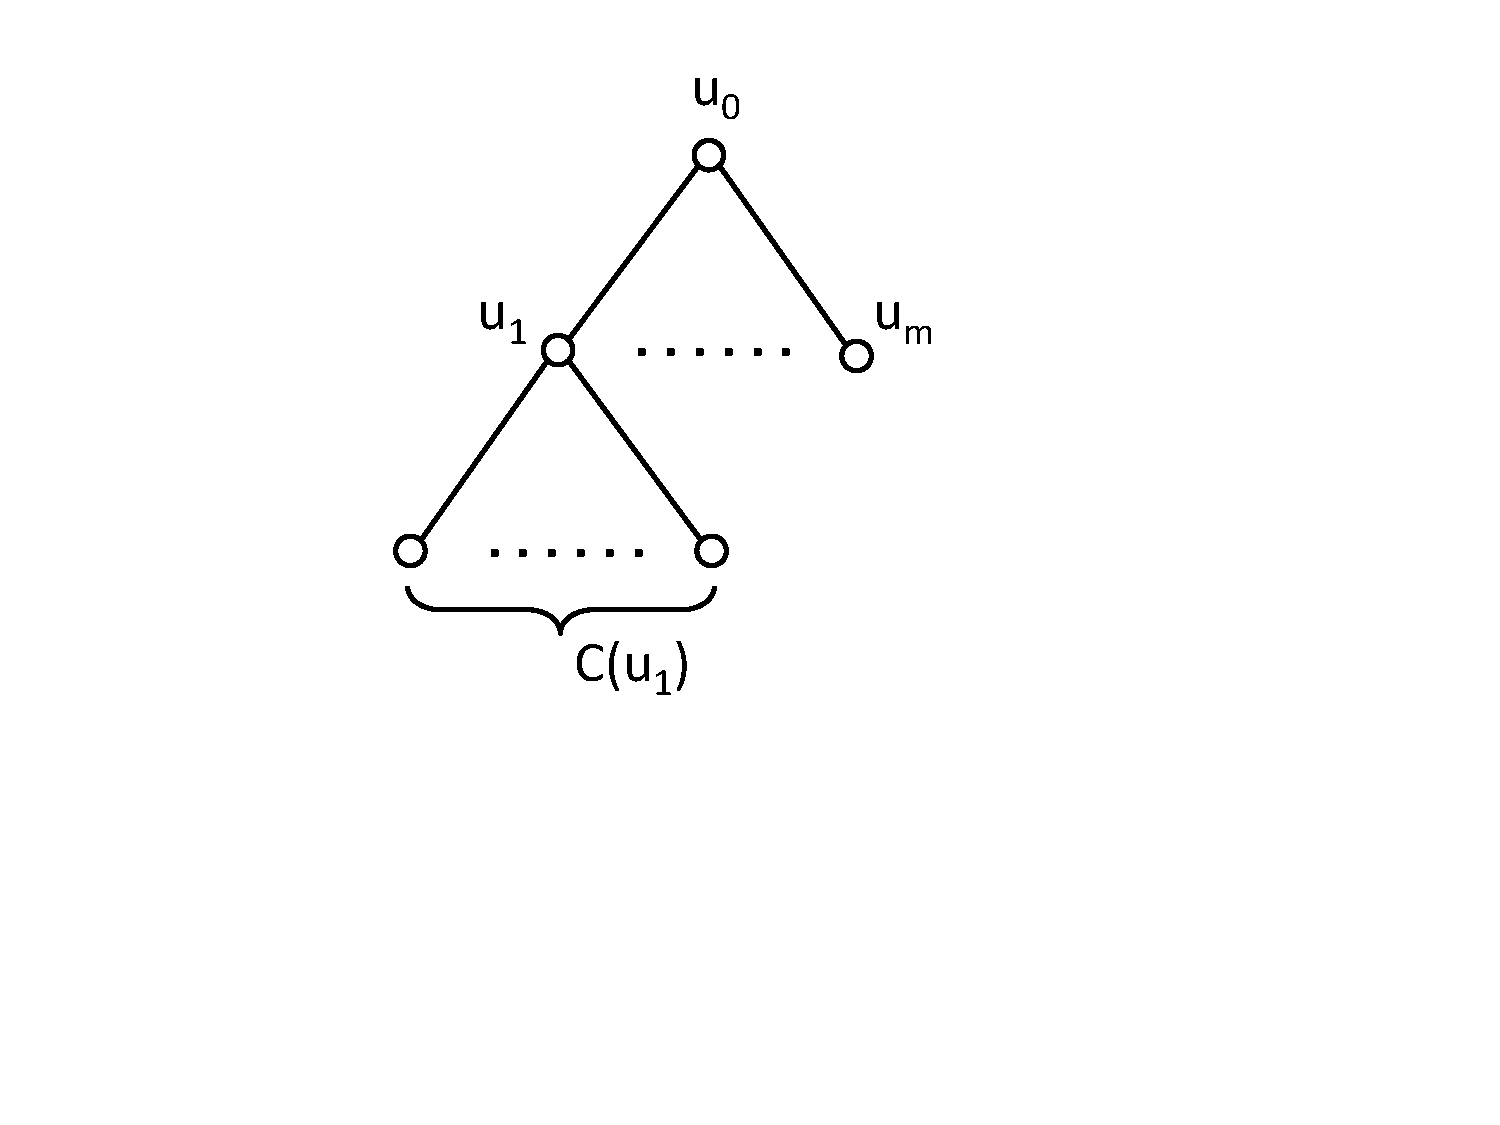
\includegraphics[scale=0.4]{../figures/fig3-2.pdf}
        \vspace{-80pt}
\caption{Minimum useful subtree of $T_{m,2}$}
\label{useful part}
\end{figure}

Now, assume the minimum span is $\lamh11(\tm2) \le 2m+h-2$. The minimum subtree contains $2m+1$ vertices that are within distance three to each other, so we need at least $2m+1$ labels to label it. More importantly, we need to have a gap with size at least $h$ between the two label sets $f(N(u_1))$ and $f(C(u_0))$. Thus in total, we need $2m+h-1$ labels to $L(h,1,1)$-label the minimum subtree of $\tm2$. This contradicts the assumption that $\lamh11(\tm2) \le 2m+h-2$. 

Lemma \ref{lem:consh11} shows that for $k = 2$, we can find an $L(h,1,1)$-labelling $f$ of $\tm2$ with $span(f) \le 2m+h-1$. Thus we are done for the minimum span of complete $m$-ary trees $\tm2$. 

By Remark \ref{construct}, we can build a complete $m$-ary tree $T_{m,k+1}$ from a complete $m$-ary tree $\tmk$. In particular, we can build $T_{m,3}$ from $\tm2$. We proved that $\lamh11(\tm2) = 2m+h-1$. Hence the minimum span $\lamh11(T_{m,3})$ is at least $2m+h-1$. However, the new vertex that is brought in when building up $T_{m,3}$ is within distance three to every other vertices in $T_{m,3}$, we must add an extra label to the original label set for $\tm2$. Thus we have $\lamh11(T_{m,3}) \ge 2m+h$. In general, we have $\lamh11(\tmk) \ge 2m+h$ for $k \ge 3$. 

It  remains to show that $\lambda_{h,1,1}(\tmk) \le 2m+h$ for $k \ge 3$. To prove this we need to find a function $f$ that $L(h,1,1)$-labels $\tmk$ such that $span(f) = 2m+h$. Though we are dealing with infinite complete $m$-ary trees, it seems when labelling these trees, there is a patten that can be followed. The idea is to pre-define two label sets. We assign one of these two label sets to each level of $\tmk$ alternatively. Precisely, we let $S_1:=[0,m], S_2:= [m+h, 2m+h]$ be two integer sets. Then the function $f$ labels $\tmk$ as follows (Fig. \ref{lh11}): 
\begin{enumerate}[(1)]
\item $f(u_0) = 0$;
\item $\{f(u_{i}) \mid i \in [1,m]\} = \SS_2 \setminus \{2m+h\}$ such that $f(u_{i}) = m+h+i-1$;
\item 
$
 f(C(u_{0\dots ijk})) =
  \begin{cases}
   \SS_1 \setminus f(P(u_{0\dots ijk})) & \text{if } d(u_0, u_{0\dots ijk}) \text{ is odd}, \\
   \SS_2 \setminus f(P(u_{0\dots ijk})) & \text{if } d(u_0, u_{0\dots ijk}) \text{ is even}. 
  \end{cases}$
\end{enumerate}

\begin{figure}
\centering
      \vspace{-10pt}
    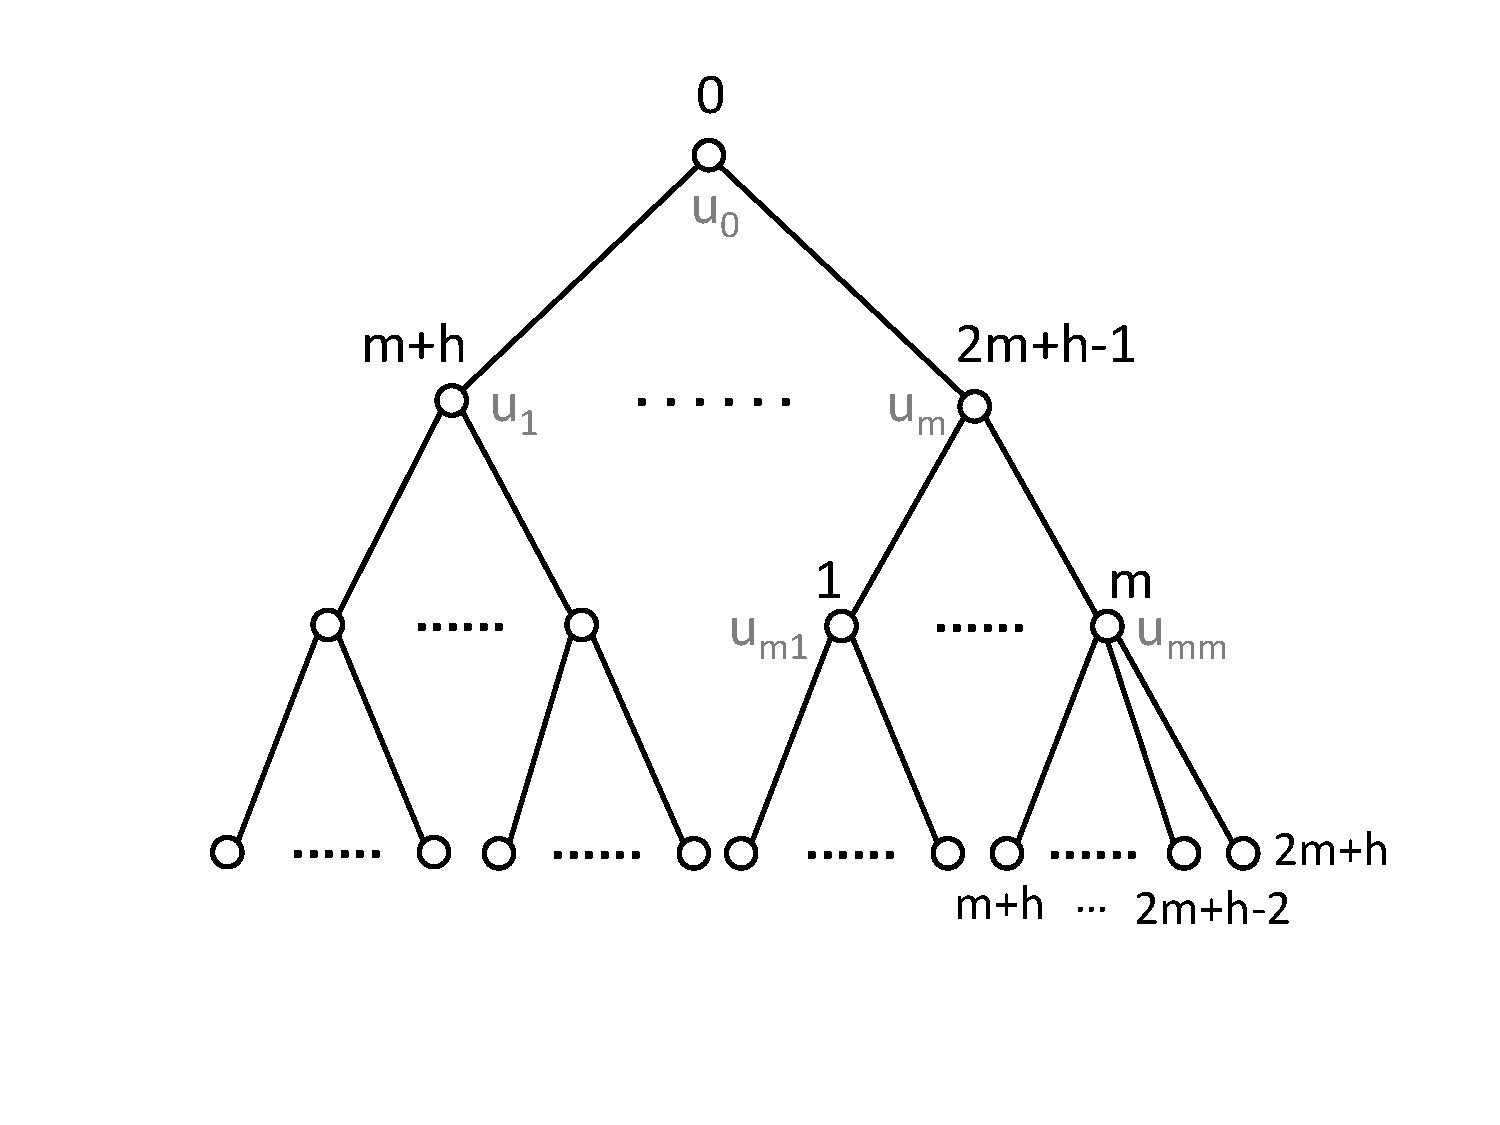
\includegraphics[scale=0.4]{../figures/fig3-3.pdf}
        \vspace{-30pt}
\caption{The $L(h,1,1)$-labelling of $T_{m,3}$ with span equals $2m+h$}
\label{lh11}
\end{figure}

It is not hard to see that $f$ perfectly $L(h,1,1)$-labels $\tmk$ with $span(f) = 2m+h$. This completes the proof of this theorem. 
\end{proof}
\qed

\begin{corollary}
\label{thm:111} For a complete $m$-ary tree $\tmk$, the minimum span of $L(1,1,1)$-labelling is 
\begin{align*}
 \lambda_{1,1,1}(\tmk) =
  \begin{cases}
   2m & \text{for } k = 2, \\
   2m+1       & \text{for } k \ge 3.
  \end{cases}
\end{align*}
\end{corollary}

This corollary agrees with Corollary $5$ in the paper published by \cite{zhou10}. They claimed that for a finite tree $T$ with diameter at least $3$ or an infinite tree with finite maximum degree, the following holds: 
\[
\chi(T^3) = \lambda_{1,1,1}(T) + 1 = \Delta_2(T).
\] 

\begin{remark}
For every tree $T$, there exits a complete $m$-ary tree $\tmk$ such that $T \subseteq \tmk$ is a subtree. Thus by the generalisation of Lemma \ref{subtree}, we have $\lamh11(T) \le \lamh11(\tmk)$ where $T \subseteq \tmk$ is a subtree. As we proved $\lamh11(\tmk)$ to be exact values, it follows that these values can be used as the upper bound for $\lamh11(T)$. Then we have the following: 
\begin{align*}
\lamh11(T) \le 
\begin{cases}
2m+h-1 & \text{ for } k =2, \\
2m+h & \text{ for } k \ge 3.
\end{cases}
\end{align*}
where $T$ is a finite tree or an infinite tree with finite maximum degree such that $diam(T) \ge 3$, and $k$ is the height of the minimal \footnote{In this case, we say the complete $m$-ary tree is minimal if it is contained in all other complete $m$-ary trees, in which $T$ is a subtree.} complete $m$-ary tree $\tmk$ that contains $T$ as a subtree. 
\end{remark} 

So far we have presented our first major theorem in this thesis. Based on this theorem, we slightly improved the upper bound stated by Theorem $1$ in \cite{zhou10}. In the next section, we will extend the $L(h,1,1)$-labelling problem to a more general and interesting version, the $\lhpq$-labelling problems.


%%%%%%%%%%%%%%%%%%%%%%%%%%%%%%%%%%%

\section{The $L(h,p,q)$-labelling of complete $m$-ary trees}

Previously, we studied the $L(h,1,1)$-labelling of complete $m$-ary trees. We found an exact value for the minimum span $\lambda_{h,1,1}(\tmk)$ of a complete $m$-ary tree $T_{m,k}$, which depends on the parameters $m$ and $h$. Surprisingly, this value is independent of the tree height apart from the fact that the value for $k = 2$ is different from that for $k \ge 3$. 

Without restricting $p$ and $q$ to be $1$, it is reasonable to believe that the $\lambda_{h,p,q}$ values of $T_{m,k}$ can also be precisely determined, though  they may have dependence upon $p$ and $q$. Notice that the only restriction we demand is $h \ge p \ge q \ge 1$.

We promised in the previous section that we will prove Lemma \ref{lem:consh11}. In the following, we will state a similar but more general lemma than Lemma \ref{lem:consh11}. The proof of Lemma \ref{lem:consh11} is a special case of the following proof, in the case $p =q=1$. 

%To make life easier, we define the following notations.
%\begin{itemize}
%\item $\AA_{1} := \{\varphi(u_{0}), \varphi(C_{u_i}) \mid \forall i \in [1,m]\}$
%\item $\AA_1' := \{\varphi(C_{u_i}) \mid \forall i \in [1,m]\}$
%\item $\AA_{2} := \{\varphi(u_{i}) \mid \forall i \in [1,m]\}$
%\item $\CC_{1} := \{\phi(u_{0}), \phi(C_{u_i}) \mid \forall i \in [1,m]\}$
%\item $\CC_{2} := \{\phi(u_{i}) \mid \forall i \in [1,m]\}$
%\end{itemize}

%We call $\AA_1, \AA_2, \CC_1, \CC_2$ {\color{red} label sets} for vertices of $T$. Now, let us begin the following lemma. 

\begin{lemma}
\label{lem:conshpq} Suppose $f$ is an $\lhpq$-labelling of a complete $m$-ary tree $\tm2$ such that the following are satisfied: 

\begin{enumerate}[(1)]
\item $f(N(u_1))$ and $f(C(u_0))$ are $p$-consecutive label sets;\footnote{$f(N(u_1)) = \alpha_1 + pI_1$ and $f(C(u_0)) = \alpha_2 + pI_2$, where $I_1, I_2$ are integer sets. In particular, when $p = 1$, a $1$-consecutive set is just a consecutive set.} 
\item $\min (\lnu) - \max(\lcu) = h$ or $\min(\lcu) - \max(\lnu) = h$. 
\end{enumerate}
Then, for any other $\lhpq$-labelling of $\tm2$, say $g$, we have 
\begin{align}
\label{minimumhpq}
span(f) \le span(g). 
\end{align}
More importantly, $span(f)$ can be found exactly and is
\begin{align}
\label{exacthpq} 
span(f)= (2m-1)p+h. 
\end{align}
\end{lemma}

As in Lemma \ref{lem:consh11}, here we only deal with $f(N(u_1))$. The following is a formal proof of this lemma. 
\\
\begin{proof}
First, let us prove \eqref{exacthpq}. Without loss of generality, assign $\{0\}$ to the root $u_0$ of $\tmk$. Then we have $\{0\} \in \lnu$. We know that $|N(u_1)| = m+1$ and $|C(u_0)| = m$, then condition (1) and (2) imply $\lnu = [0,m]p$ and $\lcu = mp+h+[0,m-1]p$. Hence, the span of the function $f$ equals the maximum label used equals $(2m-1)p+h$. 

To prove \eqref{minimumhpq}, we need to study the function $g$ that satisfies various conditions. The easiest case is when $g$ satisfies both $(1)$ and $(2)$. Then \eqref{minimumhpq} holds, as $span(f) = span(g)$. 

It remains to check that \eqref{minimumhpq} always holds even if $g$ fails to obey at least one of the above two conditions. Without loss of generality, we assume $0 \in g(N_{u_1})$ for all the following cases. 
\\
\textbf{Case $1$.} The labelling $g$ satisfies condition $(1)$ but not $(2)$. 

(1) implies $\gnu= [0, m]p$. Since condition $(2)$ is not satisfied by $g$, we have $\min\{\gcu\} - \max\{\gnu\} \ge h+1$. By consecutiveness of $\gcu$, we have $\gcu = a+[0,m-1]p$, where $a \ge mp+h+1$. Thus, 
\begin{align*}
span(g) &= a+(m-1)p \\
&\ge (2m-1)p+h+1 \\
&> (2m-1)p+h\\
&= span(f).
\end{align*}
\textbf{Case $2.1$.} The labelling $g$ does not satisfy conditions $(1)$ and \\$[0, \max\{\gnu\}] \cap \gcu = \emptyset$. 

As condition $(1)$ is not satisfied, we have at least one of $\gnu$ and $\gcu$ is not consecutive. Without loss of generality, let us assume $\gnu$ is not consecutive. In this case, we have $\gnu \subsetneq [0, \max\{\gnu\}]$. From Case 1, we know that if $\gnu$ is consecutive, then $\gnu = [0,m]p$, so here we must have $\max\{\gnu\} > mp$ if $\gnu$ is not consecutive. Since it is not sure whether condition $(2)$ is satisfied, then for $g$ to $\lhpq$-label $\tm2$, we have 
$$\min\{\gcu\} -\max\{\gnu\} \ge h$$ 
provided $[0, \max\{\gnu\}] \cap \gcu = \emptyset$. Moreover, as the consecutiveness of $\gcu$ is unknown, we have
$$\gcu \subseteq [\min\{\gcu\}, \max\{\gcu\}],$$ 
where 
\begin{align*}
&\min\{\gcu\} \ge \max\{\gnu\}+h 
\intertext{and}
&\max\{\gcu\} \ge \min\{\gcu\}+(m-1)p. 
\end{align*}
Hence we have 
\begin{align*}
span(g) &= \max\{\gcu\} \\
&\ge \min\{\gcu\}+(m-1)p \\
&\ge \max\{\gnu\}+h+(m-1)p \\
&> mp+h+(m-1)p \\
&= (2m-1)p+h \\
&= span(f).
\end{align*}
\textbf{Case $2.2$.} The labelling $g$ does not satisfy condition $(1)$ and\\ $[0, \max\{\gnu\}] \cap \gcu \neq \emptyset$. 

First, let  
$I :=  [0, \max\{\gnu\}] \cap \gcu$ be the intersected part. By condition of Case 2.2, we have $|I| \neq 0$. 

%The map $g$ is an $\lhpq$-labelling of $\tm2$ ensures that $\gnu \cap \gcu = \emptyset$. Then we have $I \subsetneq \gcu$ is a proper subset. 

The violation of condition (1) implies at least one of $\gnu$ and $\gcu$ is not consecutive. Also, as $d(u,v) = 1$ for any vertices $u \in \gnu, v \in \gcu$, then $\gnu \cap \gcu = \emptyset$. We have assumed that $\{0\} \in \gnu$, then it is not possible for $\gnu$ to be consecutive, for otherwise $|I| = 0$. It is obvious that the more pieces $\gnu$ or $\gcu$ has, the larger $span(g)$ will be. Therefore, the smallest span is achieved in the case where $\gnu$ consists of two pieces and $\gcu$ is consecutive; i.e., $\gcu \subsetneq [0, \max\{\gnu\}]$. If we can prove that $span(g)$ obtained in this case is still no less than $span(f)$, then \eqref{minimum} is true. 
Let 
\begin{align*}
&\gnu = \gnu^1 \cup \gnu^2\\
\intertext{and} 
&S = [0, \max\{\gnu\}],
\end{align*}
where $\gnu^1$ and $\gnu^2$ are both consecutive label sets. 

Since $g$ is an $L(h,1,1)$-labelling of $\tm2$ and condition (2) is unknown, there exits two forbidden gaps\footnote{The part of labels that cannot be used when $L(h,1,1)$-label $\tm2$ is said to be forbidden gaps.} $\GG_1, \GG_2$ in between the sets $\gnu^1, \gcu$ and $\gcu, \gnu^2$ with cardinalities $|\GG_1| \ge h-1$ and $|\GG_2| \ge h-1$. Thus we have (Fig. \ref{case2.2})
\begin{align*}
S &= \gnu^1 \cup \GG_1 \cup \gcu \cup \GG_2 \cup \gnu^2. 
\end{align*}
This implies 
\begin{align*}
\max\{\gnu\}
&\ge (2m-2)p+2h.
\end{align*}
Note that $((2m-2)p+2h) - ((2m-1)p+h) = h-p \ge 0$, as $h \ge p$. Then we have $span(g) \ge span(f)$. This completes the proof of this lemma. 
\begin{figure}
\centering
      \vspace{-5pt}
    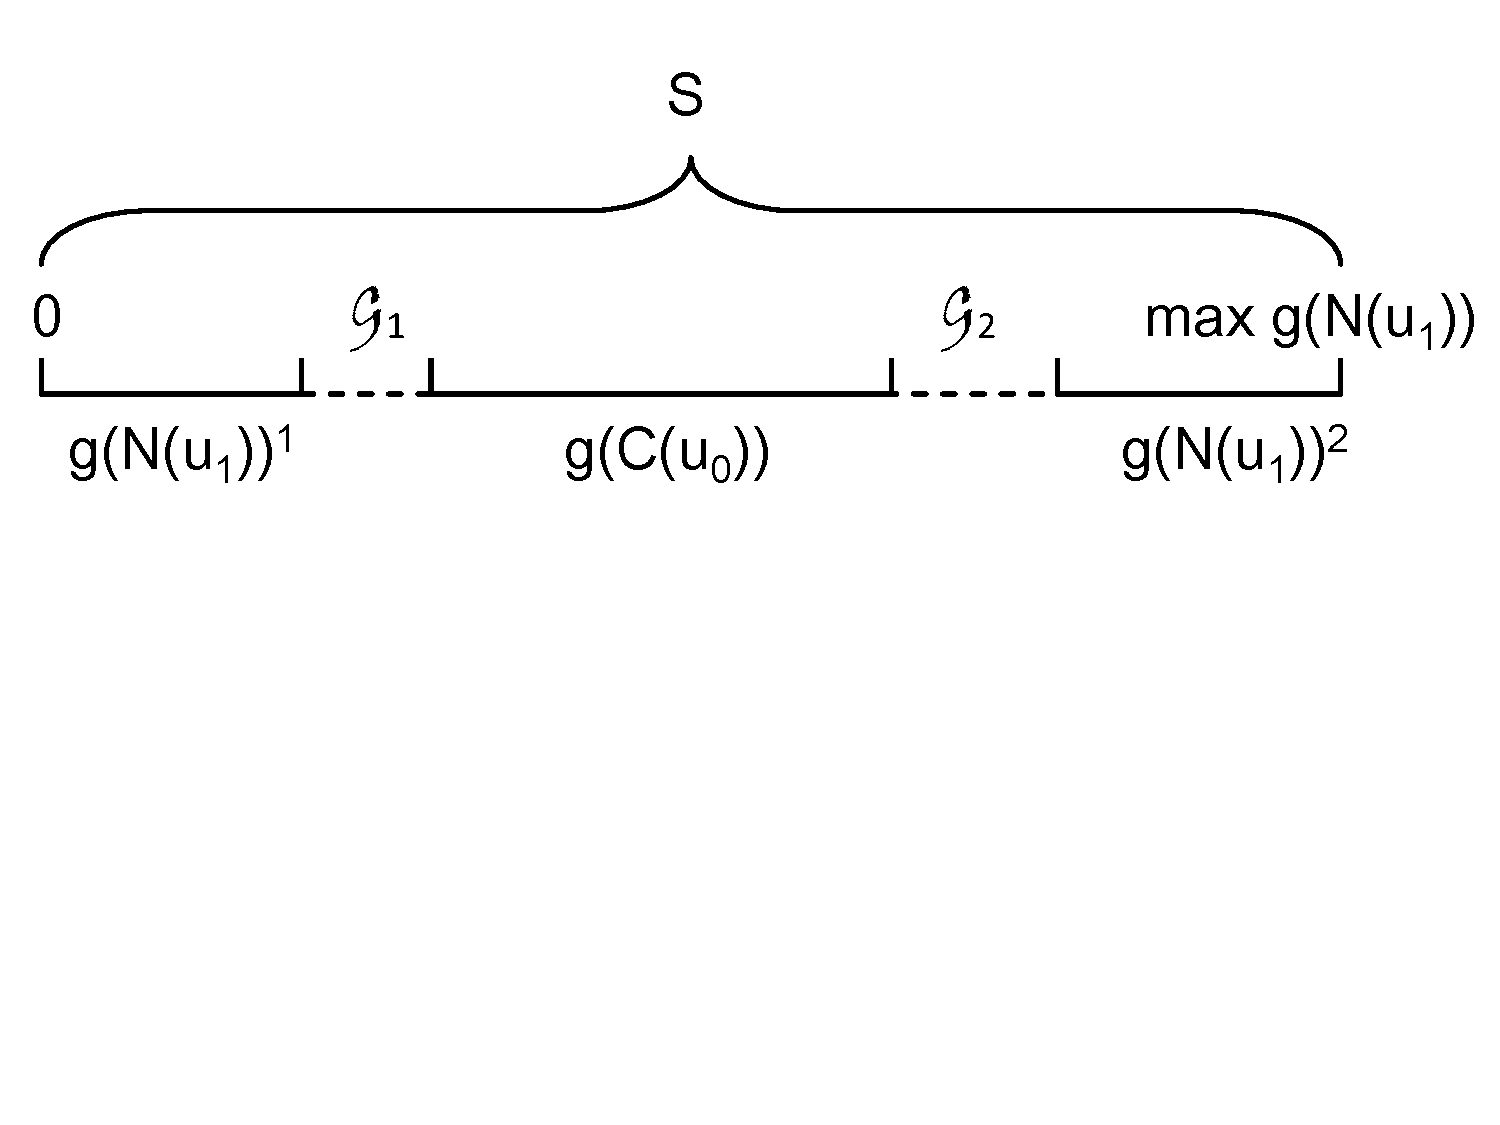
\includegraphics[scale=0.4]{../figures/fig3-4.pdf}
        \vspace{-110pt}
\caption{$\gcu \subsetneq [0, \max\{\gnu\}]$}
\label{case2.2}
\end{figure}
\end{proof}
\qed


\begin{remark}
\label{hpqtm2}
For any $L(h,p,q)$-labelling of a complete $m$-ary tree $\tm2$ under the conditions in Lemma \ref{lem:conshpq}, \eqref{minimumhpq} is always true. This implies the minimum span $\lamhpq(\tm2) \le span(f) = (2m-1)p+h$. On the other hand, it is not hard to see that to $\lhpq$-label $\tm2$, the minimum required label set is $[0, 2m-1]p+h$, so $\lambda_{h,p,q}(\tm2) \ge (2m-1)p+h$. Hence we have  
\begin{align}
\label{minispanhpq}
\lambda_{h,p,q}(T) = (2m-1)p+h.
\end{align}

\end{remark}


\begin{theorem}
\label{thm:hpq}
Let $h \ge p \ge q \ge 1$. For a complete $m$-ary tree $\tmk$, the minimum span of the $\lhpq$-labeling is
\begin{align}
\label{eq:thmhpq}
\lambda_{h,p,q}(\tmk) = 
 \begin{cases}
 (2m-1)p+h & \text{ when } k = 2, \\
 2mp+h & \text{ when } k \ge 3.
 \end{cases}
\end{align}
\end{theorem}

Substitute $p=q=1$ into \eqref{eq:thmhpq}, we get the same result as Theorem \ref{thm:h11}, that is, the minimum span of the $L(h,1,1)$-labelling of complete $m$-ary trees $\tmk$ is
\begin{align*}
 \lambda_{h,1,1}(\tmk) =
  \begin{cases}
   2m+h-1 & \text{for } k = 2, \\
   2m+h       & \text{for } k \ge 3.
  \end{cases}
 \end{align*}
In other words, Theorem \ref{thm:h11} is a special case of Theorem \ref{thm:hpq}. The proof of this theorem is similar to the proof of Theorem \ref{thm:h11}. We will first prove \eqref{eq:thmhpq} is a lower bound. Then we will construct specific $\lhpq$-labelling for $\tmk$ with span equals \eqref{eq:thmhpq}.  

Notice that this theorem claimed that the $\lamhpq$ value is independent of the third parameter $q$. This is due to the restriction $h \ge p \ge q \ge 1$. 
\\
\begin{proof}
Remark \ref{hpqtm2} proved that $\lamhpq(\tm2) = (2m-1)p+h$. Now, we want to show that $\lamhpq(\tmk) \ge 2mp+h$ for $k \ge 3$. 

We mentioned before that a complete $m$-ary tree $T_{m, 3}$ can be constructed from $\tm2$ by connecting one extra vertex to roots $\{u_0^1, \dots, u_0^m\}$ of $m$ copies of $\tm2$. During this construction, we introduced a new vertex $u_0$, which is within distance $3$ to every vertex in $m$ copies of $\tm2$. Then the minimum span $\lamhpq(T_{m,3}) \ge \lamhpq(\tm2) + p$. Thus we have $\lamhpq(\tmk) \ge \lamhpq(T_{m,3}) \ge 2mp+h$ for $k \ge 3$. 

It is remaining to show that \eqref{eq:thmhpq} is also the upper bound of $\lamhpq(\tmk)$ for $k \ge 3$. To prove this, we will construct similar labelling system as those before for $L(h,1,1)$-labelling of $\tmk$. 

Define $\SS_1: = [0,m]p$ and $\SS_2 := (mp+h)+[0,m]p$ to be the label sets we need. Below we provide details of how to $\lhpq$-label $\tmk$ for $k \ge 3$. 
\begin{enumerate}[(1)]
\item $f(u_0) = 0$;
\item $\{f(u_i) \mid i \in [1,m]\} = \SS_2 \setminus \{2mp+h\}$ such that $f(u_i) =(m+i-1)p+h$;
\item $f(C(u_{0 \dots ijk})) =
 \begin{cases}
 \SS_1 \setminus f(P(u_{0 \dots ijk})) & \text{ if } d(u_0, u_{0\dots ijk}) \text{ is odd, } \\
 \SS_2 \setminus f(P(u_{0 \dots ijk})) & \text{ if } d(u_0, u_{0\dots ijk}) \text{ is even.} 
 \end{cases}$
\end{enumerate}

Clearly $f$ is an $\lhpq$-labelling of $\tmk$ with $span(f) = 2mp+h$. This completes the proof of Theorem \ref{thm:hpq}. 
\end{proof}
\qed




%%%%%%%%%%%%%%%%%%%%%%%%%%%%%%%%%%%

\section{The $L(h,p,q)$-labelling of broader sets of trees}

From now on, we will generalise our $\lambda_{h,p,q}$ results to a more general set of trees, which contains the set of complete $m$-ary trees as a proper subset. 

We recall some notation defined earlier. We use $\Delta(T)$ (or $\Delta$) to denote the maximum degree of a tree $T$, the term $\Delta_2(T)$ (or $\Delta_2$) to denote the sum of the degrees of an heavy edge; $\Delta_2(T) := \max_{uv \in E(T)}((d(u) + d(v))$.
%%%%%%%%%%%%%%%%%%%%%%%%%%%%%%%%%%%




\subsection{The sets of trees with $\Delta_2$ value equals $2\Delta-1$ or $2\Delta$}
\label{sec:general sets}

To start, let us define the following: 
\begin{itemize}
\item Let $\TT := \{\tmk \mid m \ge 2, k\ge 2\}$ be the set of complete $m$-ary trees with $m, k \ge 2$.
\item Let $\TT^{(n)} := \{\tmk \in \TT \mid k=n\}$ be the set of complete $m$-ary trees with height exactly $n$. 
\item Let $\TT^{(\ge n)} := \{\tmk \in \TT \mid k \ge n\}$ be the set of complete $m$-ary trees with height no less than $n$. 
\item $\DD := \{T \mid diam(T) \ge 3, \Delta_2(T) = 2\Delta-1 \}$. 
\item $\FF := \{T \mid diam(T) \ge 3, \Delta_2(T) = 2\Delta\}$. 
\end{itemize}

Notice that $\TT^{(2)} \subsetneq \DD$ and $\TT^{(\ge 3)} \subsetneq \FF$ are proper subsets of the sets $\DD$ and $\FF$ respectively. The following corollary gives a bound on $\lamh11$ values of the sets $\DD$ and $\FF$ based on the $\lamh11$ value of complete $m$-ary trees $\tmk$. 

\begin{corollary}
\label{cor:subtree}
For any tree $D \in \DD$ or $F \in \FF$, we can find a complete $m$-ary tree $\tmk$ such that 
\begin{align*}
\lambda_{h,p,q}(\tmk) \ge
  \begin{cases}
   \lambda_{h,p,q}(D), \\
   \lambda_{h,p,q}(F).
  \end{cases}
 \end{align*}
 
 \end{corollary}
 
\begin{proof}
This follows from the fact that every tree $T$ is a subtree of a complete $m$-ary tree, and the subtree has the minimum span no bigger than the original tree for $L(h,p,q)$-labelling. 
\end{proof}
\qed

%It is trivial that every tree $D \in \DD$ or $F \in \FF$ is a subtree of a complete $m$-ary tree $\tmk$. However, it does not help if we find an arbitrarily large $\tmk$ that covers $D$ or $F$, as our aim is to reduce the upper bound of $\lamhpq(D), \lamhpq(F)$ as much as possible. 

%\begin{proposition}
%\label{choosetmk}
%Let $u \in V(D), v \in V(F)$ be vertices with degrees $d_D(u) < \Delta$ and $d_F(v) < \Delta$ respectively. If letting $u$ and $v$ be the root of $D$ and $F$ respectively, then the $\lamhpq$ value of the complete $m$-ary tree that contains $D$ and $F$ are smaller than that obtained when letting a vertex with maximum degree be the root of $D$ and $F$. 
%\end{proposition} 

%\begin{proof}
%Let $u' \in V(D)$ and $v' \in V(F)$ be vertices with degrees $d_D(u') = d_F(v')= \Delta$. Theorem \ref{thm:hpq} proves that 
%\[
%\lamhpq(\tmk) = 
%\begin{cases}
%2m+h-1, & \text{for } k =2,\\
%2m+h, & \text{for } k \ge 3.
%\end{cases}
%\]
%So even if letting a vertex with the maximum degree to be the root can decrease the height of $D$ or $F$, the number of children $m$ then has to be increased by at least $1$. This follows by the result that the $\lamhpq$ value increases by at least $2$. In total, the minimum span will be increased by at least $1$. 
%\end{proof} \mymargin{fill in more details in the proof}
%\qed

%From now on, when considering the complete $m$-ary tree that contains $D$ or $F$ as a subtree, we will re-assign the root of $D$ or $F$ if the original root has maximum degree in order to achieve the least upper bound for the $\lamhpq$ values. 

\begin{definition}
\label{def:minimal}
A tree $D \in \DD$ and $F \in \FF$ is said to be minimal if $D$ and $F$ is contained as a subtree in any other trees in the set $\DD$ and $\FF$. We use $D_{min}$ and $F_{min}$ to denote the minimal trees in sets $\DD$ and $\FF$. (Fig. \ref{fig mini})
\end{definition}
\begin{figure}
\centering
      \vspace{-10pt}
    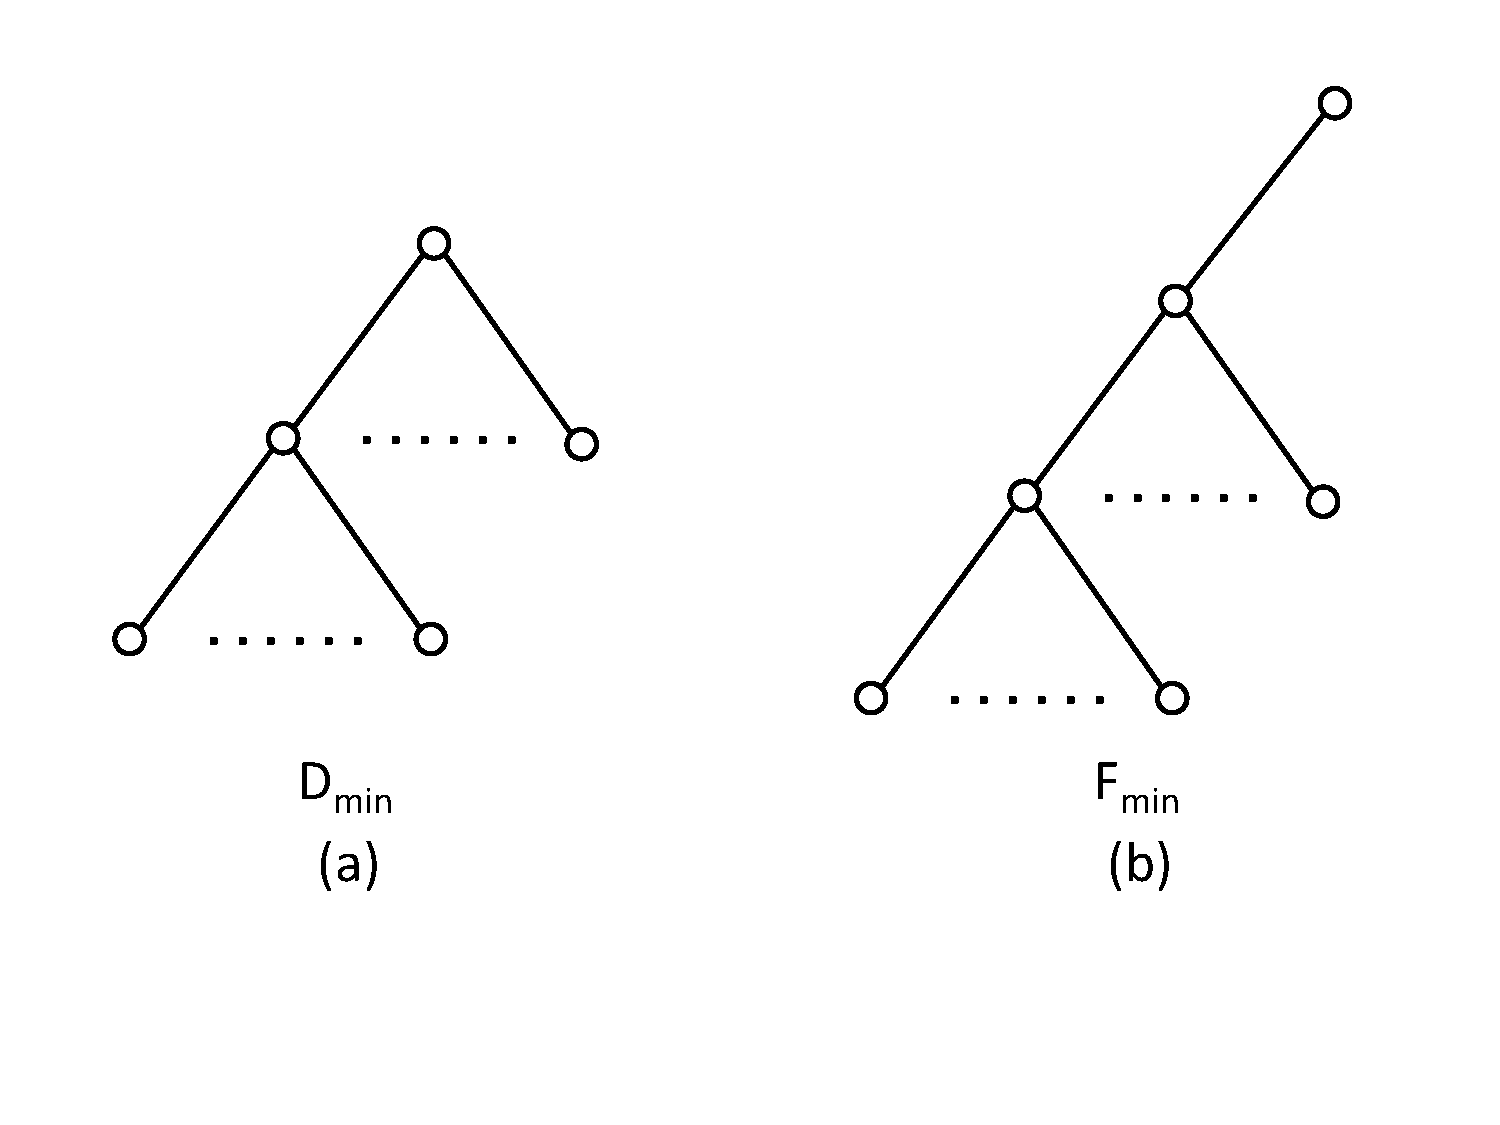
\includegraphics[scale=0.4]{../figures/fig3-5.pdf}
        \vspace{-40pt}
\caption{The minimal trees $D_{min} \in \DD$ and $F_{min} \in \FF$}
\label{fig mini}
\end{figure}

\begin{definition}
\label{def:maximal}
A tree $D \in \DD$ and $F \in \FF$ is said to be maximal if $D$ and $F$ contains all other trees in the set $\DD$ and $\FF$ as subtrees. 
\end{definition}


\begin{remark}
\label{rmk:mini}
By definition of the minimal tree, we have  
\begin{align*}
D_{min} \subseteq D \text{ and }
%\intertext{and}
F_{min} \subseteq F,
\end{align*}
for all $D \in \DD$ and $F \in \FF$. This implies that 
\begin{align*}
\lamhpq(D_{min}) \le \lambda_{h,p,q}(D) 
\intertext{and}
\lamhpq(F_{min}) \le \lambda_{h,p,q}(F). 
\end{align*}
\end{remark}








%%%%%%%%%%%%%%%%%%%%%%%%
\subsection{Generalisation of the $\lhpq$-labelling problem to the sets $\DD$ and $\FF$}
\label{sec:general results}

In the previous studies, we solved the $L(h,1,1)$ as well as the $\lhpq$-labelling problems of complete $m$-ary trees. As the former is a special of the latter, we did not spend too much time on proofs of the $\lhpq$-labelling results. Now, instead of generalising the $L(h,1,1)$-labelling result from complete $m$-ary trees to sets $\DD$ and $\FF$, we will generalise the $\lhpq$-labelling results to these sets. The $L(h,1,1)$-labelling result can then be seen as a corollary to these results. 
\begin{corollary}
\label{cor:ub}
For any trees $D \in \DD$ and $F \in \FF$, the minimum spans of the $L(h,p,q)$-labelling are bounded by
\begin{align}
\label{upper1}
\lambda_{h,p,q}(D) &\le (2\Delta -3)p+ h\\
\intertext{and}
\label{upper2}
\lambda_{h,p,q}(F) &\le (2\Delta-2)p + h. 
\end{align} 
Moreover, these bounds are the least upper bounds for $\lamhpq$ values. 
\end{corollary}

\begin{proof}
It is easy to see that these upper bounds are indeed the smallest possible, as $\TT^{(2)} \subsetneq \DD$ and $\TT^{(\ge 3)} \subsetneq \FF$ are proper subsets. If these bounds could be decreased, we would contradict Theorem \ref{thm:hpq}. 

By definitions of  the sets $\DD$ and $\FF$, we have the height of any tree $D \in \DD$ is no less than $2$, and the height of any tree $F \in \FF$ is no less than $3$. Now, substituting $m = \Delta-1$ into Theorem \ref{thm:hpq} the result is 
\begin{align}
\lambda_{h,p,q}(\tmk) = 
 \begin{cases}
 (2\Delta-3)p + h & \text{ for } k=2, \\
 (2\Delta-2)p + h & \text{ for } k \ge 3. 
 \end{cases}
\end{align} 
By Corollary \ref{cor:subtree}, we then get 
\begin{align*}
%\label{ubforD}
\lambda_{h,p,q}(D) &\le 
 \begin{cases}
 (2\Delta-3)p + h  & \text{ for } hei(D) = 2, \\
 (2\Delta-2)p + h & \text{ for } hei(D) \ge 3. 
 \end{cases} \\
\intertext{and}
\lambda_{h,p,q}(F) &\le (2\Delta-2)p + h, \forall F \in \FF. 
\end{align*} 

It remains to show that the upper bound can be decreased by $p$ when $hei(D) \ge 3$; i.e., $\lambda_{h,p,q}(D) \le (2\Delta-3)p+h$, for $hei(D) \ge 3$. 

Notice that for a tree $D \in \DD$ with $hei(D) \ge 3$, we must not have $\Delta_2(D) = 2\Delta$. This is due to the definition of the set $\DD$. Hence, the maximal tree $D_{max}$ must satisfy the following property: 
\begin{enumerate}[(*)]
\item for any heavy edge $uv \in E(D)$, we must have $d(u) = \Delta, d(v) = \Delta-1$ or $d(v) = \Delta, d(u) = \Delta-1$. 
\end{enumerate}

The upper bound $(2\Delta-2)p+h$ comes from Theorem \ref{thm:hpq} for complete $m$-ary tree $\tmk$ with $k \ge 3$. We have proved that to $L(h,p,q)$-label $\tmk$, we alternatively assign label sets $S_1=[0,m]p$ and $S_2=(mp+h)+[0,m]p$ to sets of vertices in each depth. But for the tree $D_{max}$, each set of vertices with either even or odd depth has one element less than those in $\tmk$ by property (*). Thus we can delete a label from label set $S_1$ or $S_2$. In either case, the minimum span is reduced by $p$. For example, if $D_{max}$ is as shown in Fig. \ref{ex D 1}, then we use the following label sets: 
\begin{itemize}
\item $S_1' = [0, m-1]p$; 
\item $S_2' = (m-1)p+h+[0,m]p$. 
\end{itemize}
If $D_{max}$ is as shown in Fig. \ref{ex D 11}, then we use the following label sets: 
\begin{itemize}
\item $S_1=[0,m]p$;
\item $S_2''=mp+h+[0,m-1]p$. 
\end{itemize}

\begin{figure}
 \centering
      \vspace{-5pt}
    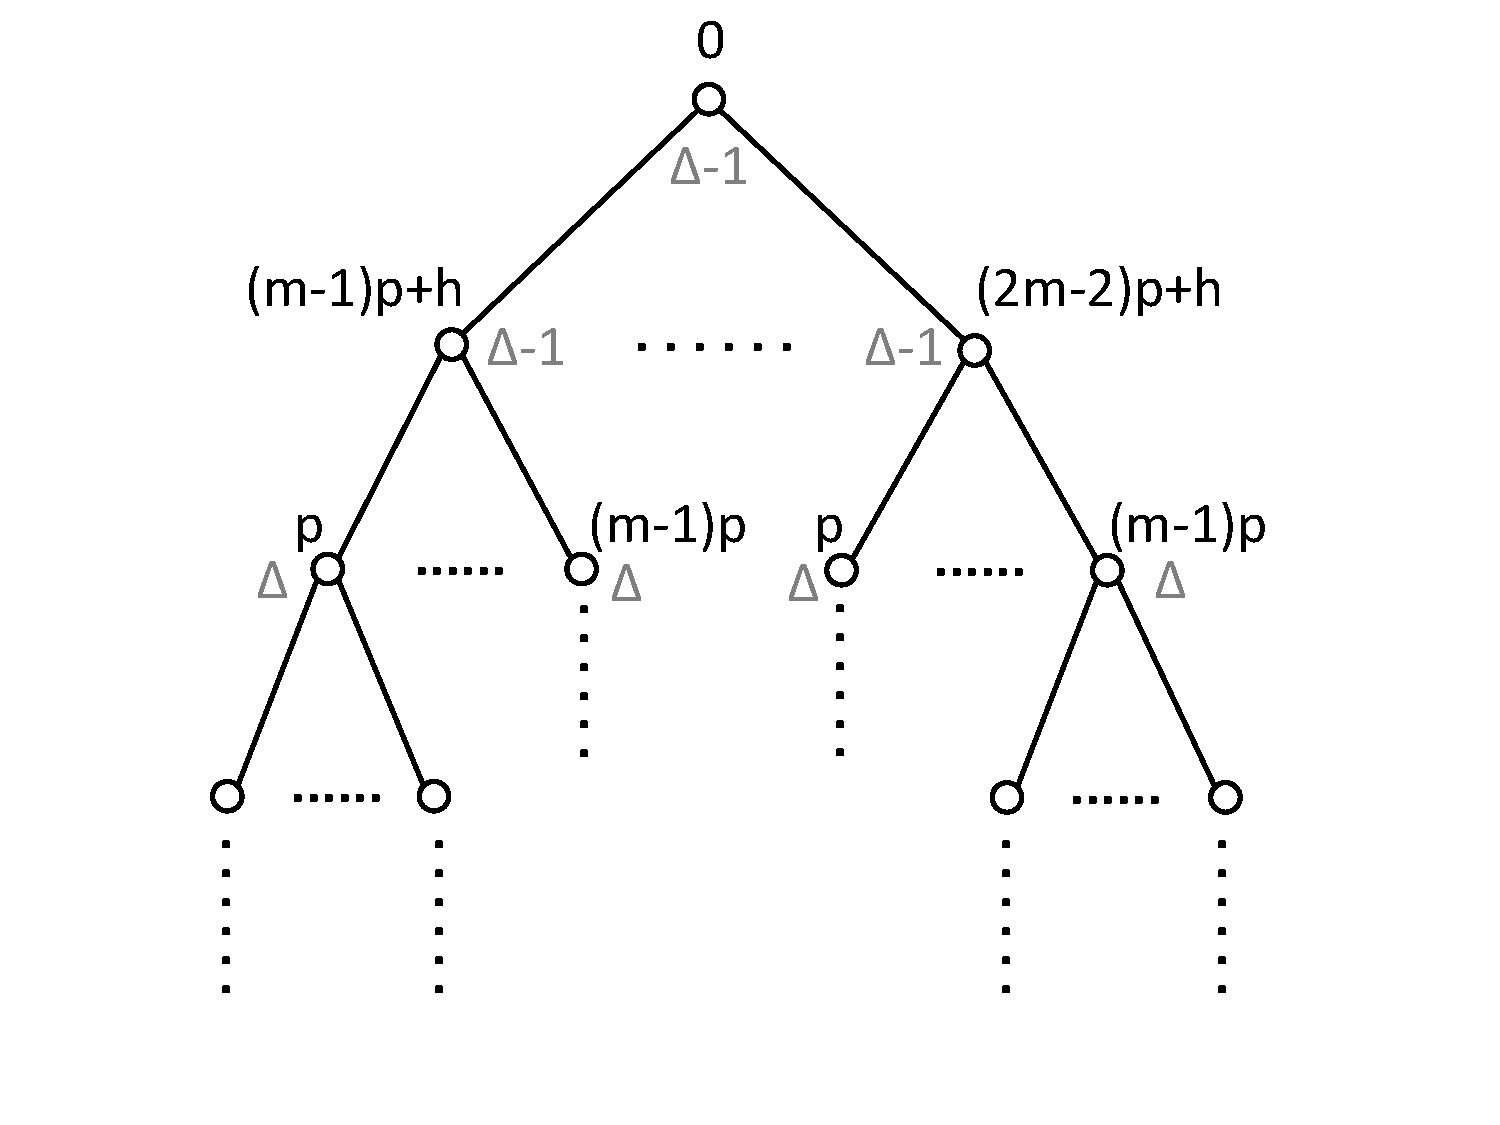
\includegraphics[scale=0.4]{../figures/fig3-6-a.pdf}
        \vspace{-0pt}
\caption{The $\lhpq$-labelling of $D_{max}$}
\label{ex D 1}
\end{figure}

\begin{figure}
 \centering
      \vspace{-20pt}
    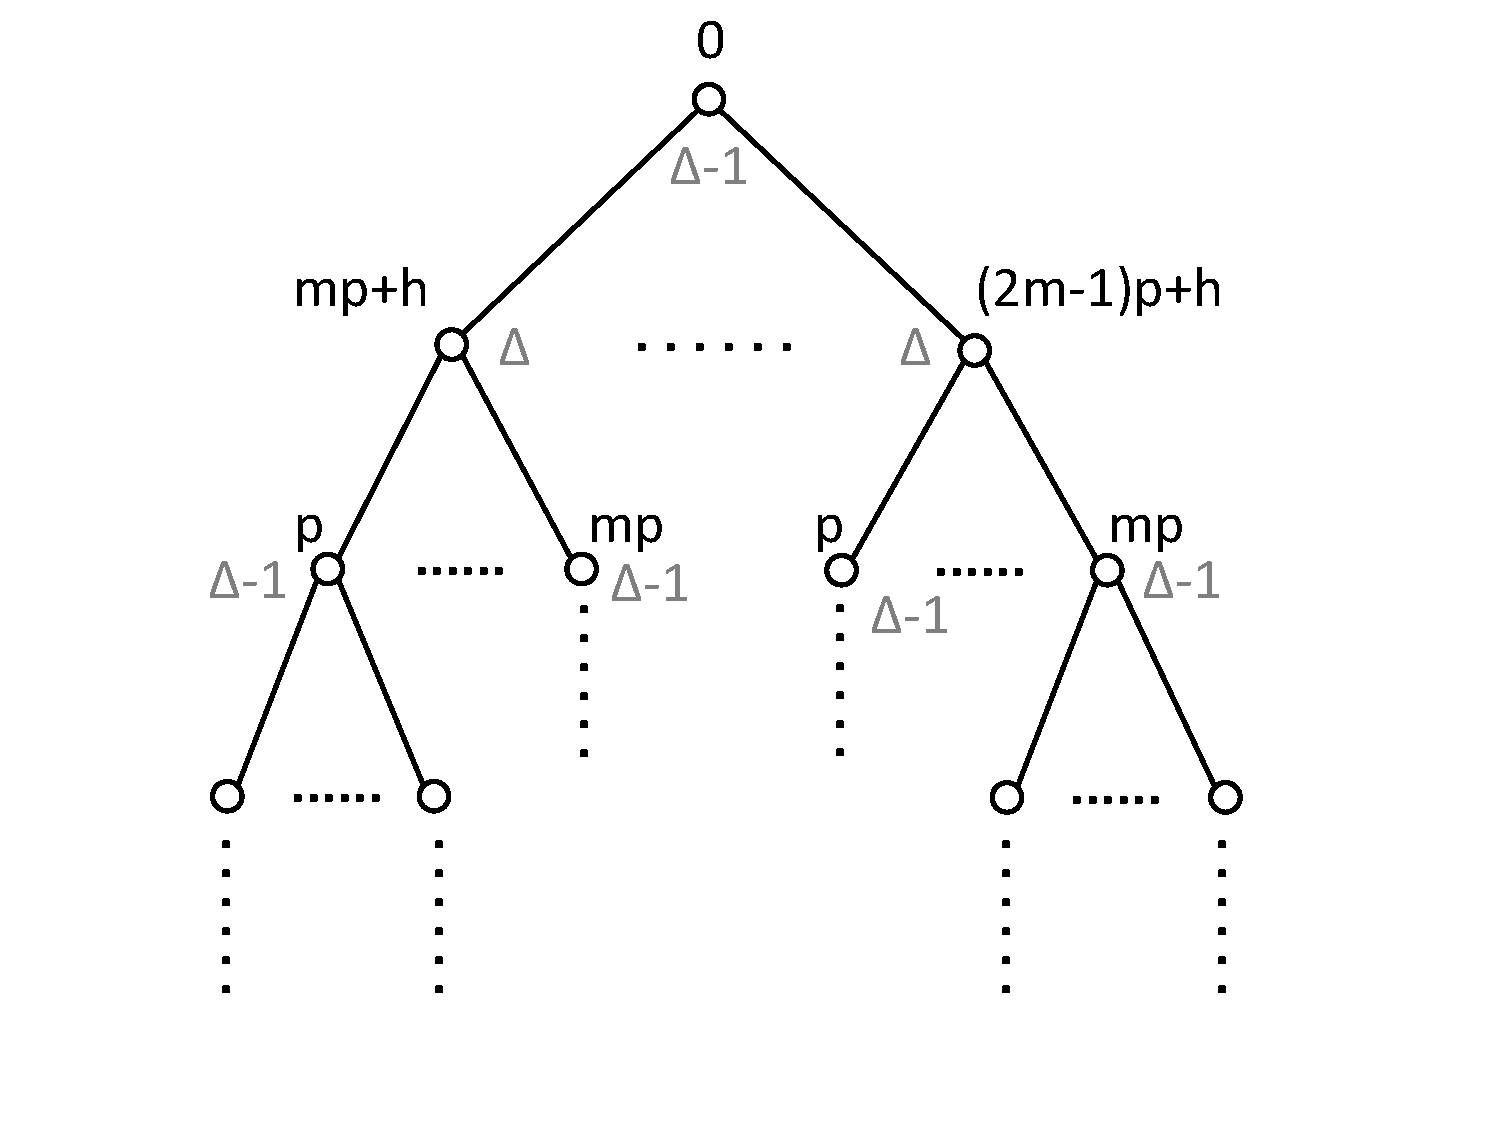
\includegraphics[scale=0.4]{../figures/fig3-6-b.pdf}
        \vspace{-0pt}
\caption{The $\lhpq$-labelling of $D_{max}$}
\label{ex D 11}
\end{figure}


By using these label sets, we showed that when $hei(D) \ge 3$, there exists a map that $L(h,p,q)$-labels $D$ with minimum span $\lambda_{h,p,q}(D) = (2m-1)p+h=(2\Delta-3)p+h$. Thus the corollary is proved.  
\end{proof}
\qed

The following two theorem gives upper and lower bounds for $\lamhpq(D)$ and $\lamhpq(F)$. 

\begin{theorem}
\label{thm:h11forD}
For any tree $D \in \DD$, the minimum span of the $\lhpq$-labelling is bounded by the following:
\begin{align*}
\max\{(2\Delta - 3)p+q, (\Delta-1)p+h\} \le \lambda_{h,p,q}(D) \le (2\Delta-3)p + h. 
\end{align*}
\end{theorem}

The value $(2\Delta-2)p+q$ is achieved for $(\Delta-2)p+q \ge h$, while $(\Delta-1)p+h$ is achieved for $(\Delta-2)p+q \le h$. 
\begin{proof}
The upper bounds have been verified by Corollary \ref{cor:ub}. it remains to prove the lower bound case by case. Remark \ref{rmk:mini} shows that $\lamhpq(D_{min}) \le \lamhpq(D)$ for all $D \in \DD$, where $D_{min} \in \DD$ is defined as the minimal tree. Thus we just need to find the $\lamhpq$  values for $D_{min}$ in each particular case. 

If $(\Delta-2)p+q \ge h$, consider $D_{min}$ with $d(u) = \Delta-1, d(v) = \Delta$. Let $f:V(D_{min}) \rightarrow [0, \infty)$ be a function, such that $f(N(v)) = [0,\Delta-1]p$ with $f(u) = 0$ and $f(N(u))=(\Delta-1)p+q+[0,\Delta-2]p$ with $f(v) = (2\Delta-3)p+q$. Then $f$ is an $L(h,p,q)$-labelling of $D_{min}$ with $span(f) = (2\Delta-3)p+q$. (Fig. \ref{ce2} (a))

If $(\Delta-2)p+q \le h$, then the function $f: V(D_{min}) \rightarrow [0,\infty)$ labels $D_{min}$ in the following way: $f(N(v))=[0,\Delta-1]p$ and $f(N(u))=p+h+[0,\Delta-2]p$ such that $f(u)=0$ and $f(v) = (\Delta-1)p+h$. Clearly, the function $f$ is again an $L(h,p,q)$-labelling of $D_{min}$ with $span(f) = (\Delta-1)p+h$. (Fig. \ref{ce2} (b))
\begin{figure}
\centering
      \vspace{-15pt}
    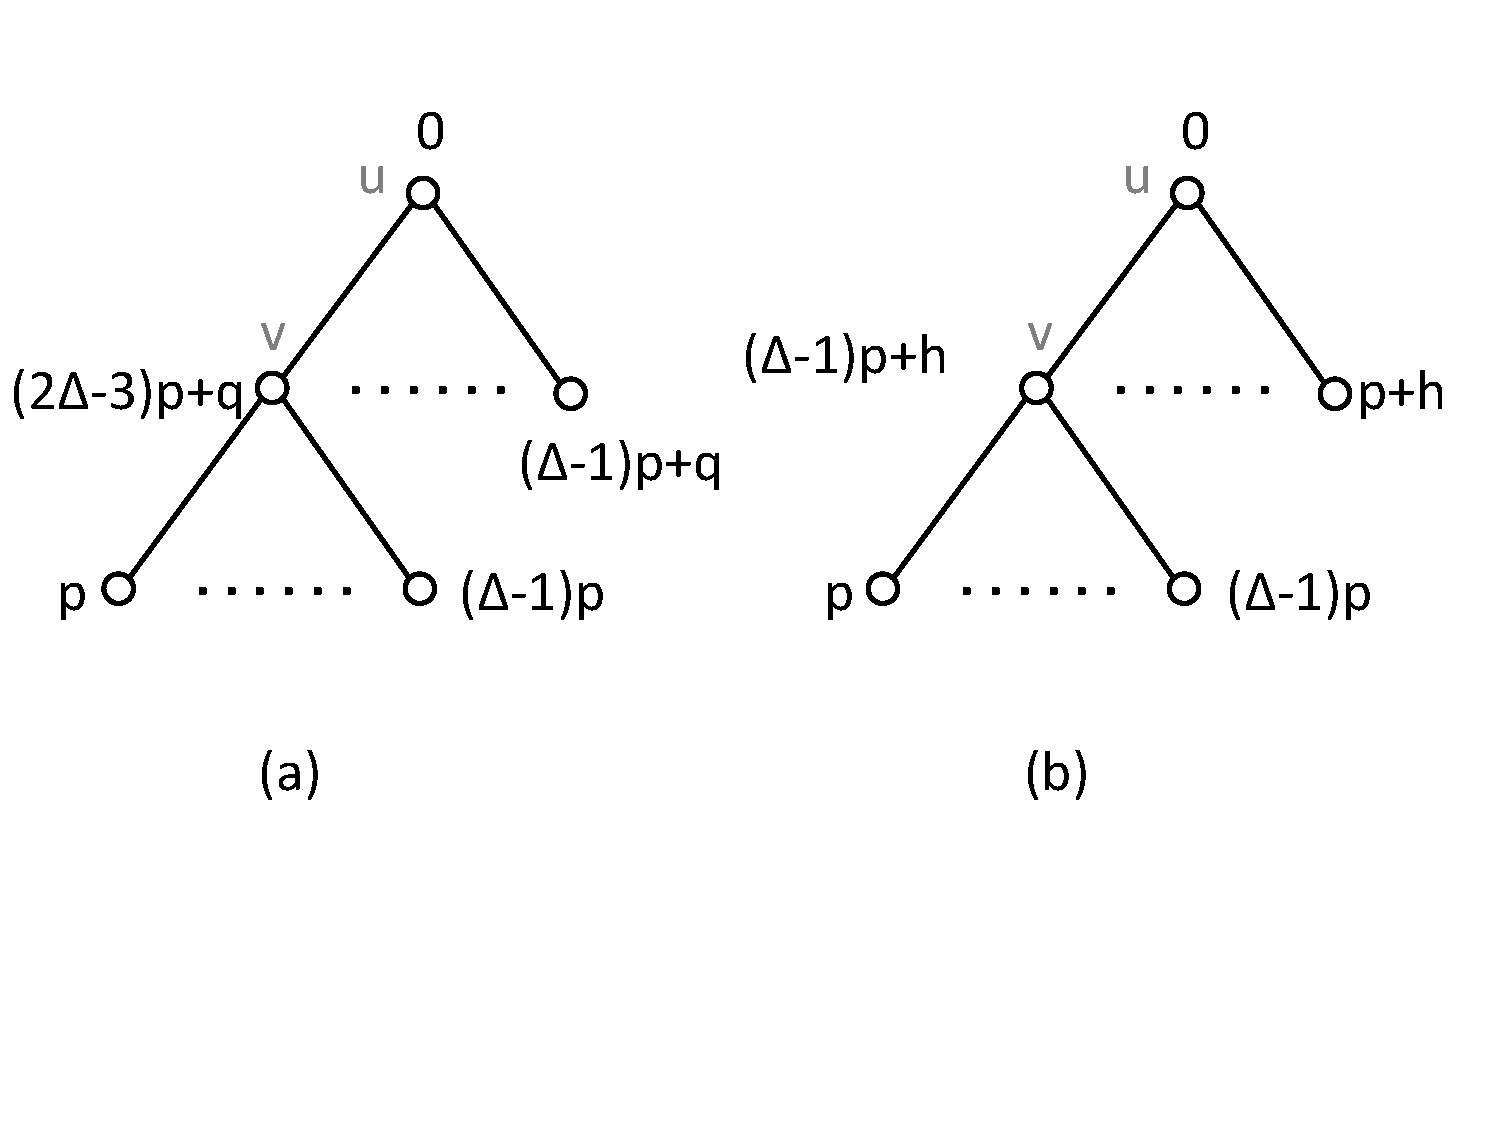
\includegraphics[scale=0.4]{../figures/fig3-7.pdf}
        \vspace{-60pt}
\caption{The $\lhpq$-labelling of $D_{min}$ with span equals $\max\{(2\Delta - 3)p+q, (\Delta-1)p+h\}$}
\label{ce2}
\end{figure}
\end{proof}
\qed

\begin{theorem}
\label{thm:h11forF}
For any tree $F \in \FF$, the minimum span of the $\lhpq$-labelling is bounded by 
\begin{align*}
\max\{(2\Delta - 2)p+q, (\Delta-1)p+h\} &\le \lambda_{h,p,q}(F) \le (2\Delta-2)p + h.
\end{align*} 
\end{theorem}

Again, the value $(2\Delta - 2)p+q$ is achieved for $(\Delta-1)p+q \ge h$, while $(\Delta-1)p+h$ is achieved for $(\Delta-1)p+q \le h$. 
\begin{proof}
The proof is similar to the proof of Theorem \ref{thm:h11forD}. We only need to prove the lower bound, as the upper bound has been proved by Corollary \ref{cor:ub}. 

Again, we solve $\lamhpq(F_{min})$ for the minimal tree $F_{min} \in \FF$. Consider a function $f:V(F_{min}) \rightarrow [0,\infty)$ such that $F_{min}$ is labelled as follows.(Fig. \ref{ce4}). 

If $(\Delta-1)p+q \ge h$, then
\begin{itemize}
\item $f\left(N(v)\right) = [0, \Delta-1]p$ such that $f(u)=0$;
\item $f\left(N(u)\right) = (\Delta-1)p+q+[0,\Delta-1]p$ such that $f(v) = (2\Delta-2)p=q$. 
\end{itemize}

If $(\Delta-1)p+q \ge h$, then 
\begin{itemize}
\item $f\left(N(v)\right) = [0, \Delta-1]p$ such that $f(u) = 0$; 
\item $f\left(N(u)\right) = h+[0,\Delta-1]p$ such that $f(v) = (\Delta-1)p+h$. 
\end{itemize}

\begin{figure}
\centering
      \vspace{-10pt}
    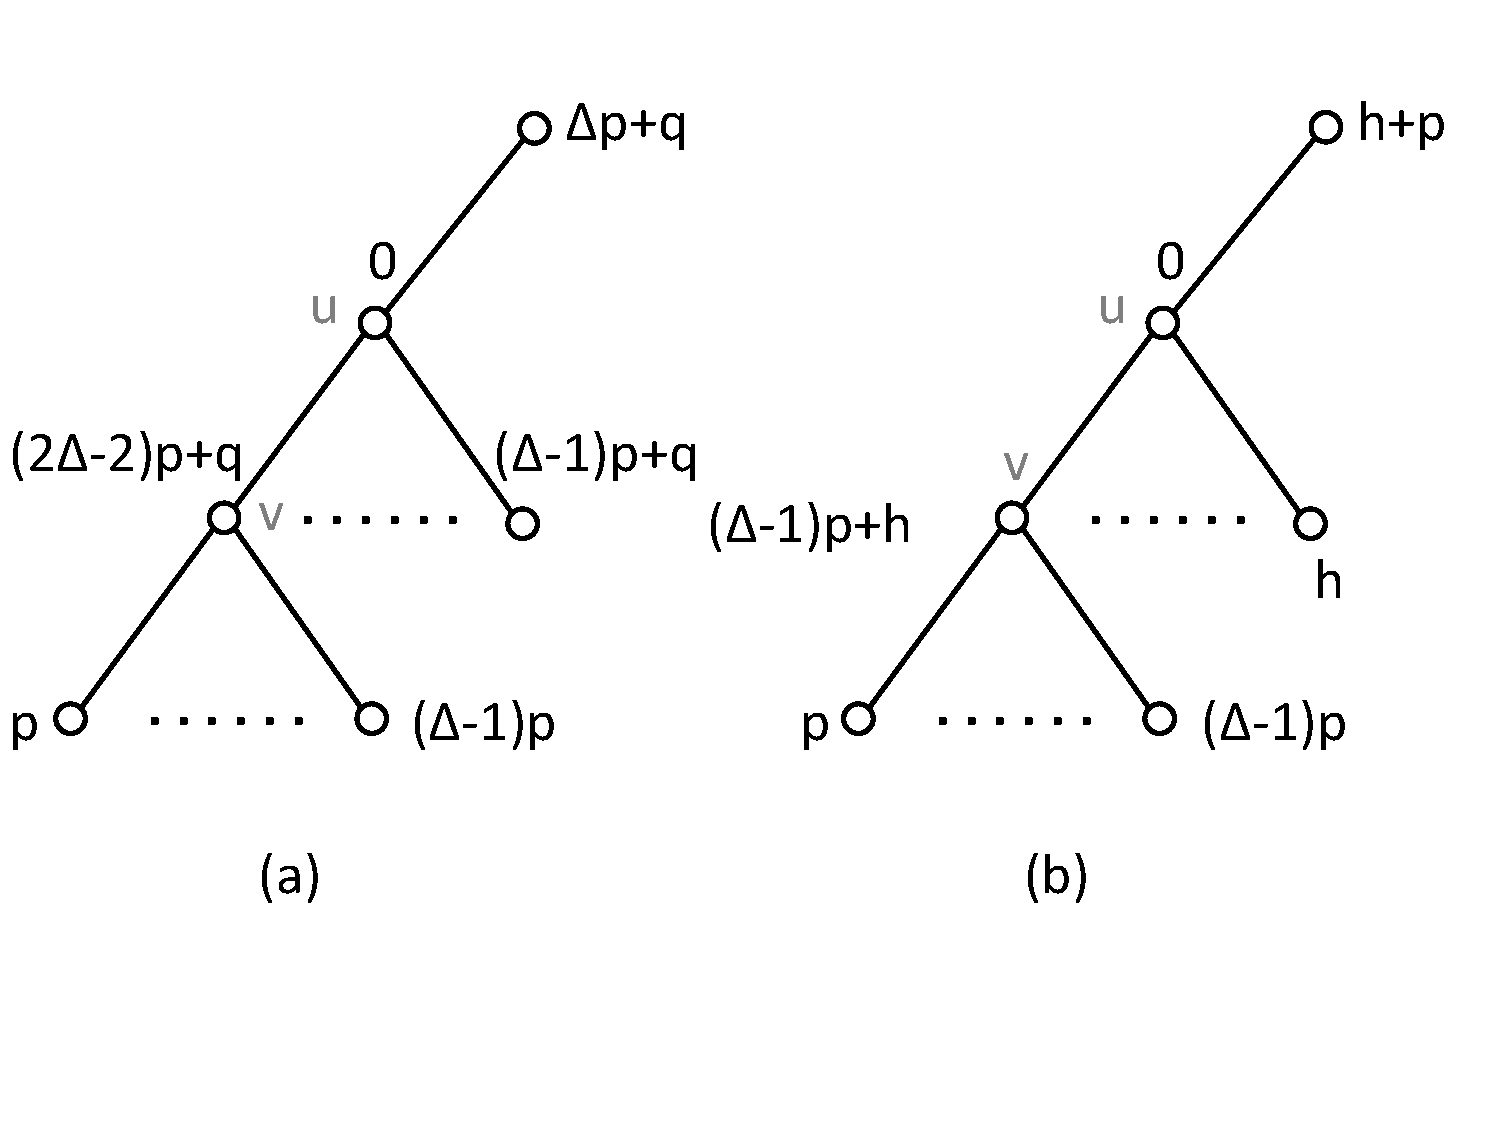
\includegraphics[scale=0.4]{../figures/fig3-8.pdf}
        \vspace{-40pt}
\caption{The $\lhpq$-labelling of $F_{min}$ with span equals $\max\{(2\Delta - 2)p+q, (\Delta-1)p+h\}$} 
\label{ce4}
\end{figure}

It can be seen that $F_{min}$ is $L(h,p,q)$-labelled by the function $f$ with $span(f) = \max\{(2\Delta - 2)p+q, (\Delta-1)p+h\}$. This completes the proof of Theorem \ref{thm:h11forF}. 
\end{proof}
\qed





%%%%%%%%%%%%%%%%%%%%%%%%%%%%%%%%%%%

\subsection{The set of trees with $T_{m,2}$ as a local structure}
\label{subsection:tm2}

Define the set 
\[
\KK :=\{ T \mid T_{m,2} \subseteq T \text{ is a subtree }, m = \Delta-1\}
\]
where $T_{m,2}$ is a complete $m$-ary tree with height $2$. We can partition this set into two subsets
\[
\KK = \KK_{2\Delta} \cup \KK_{2\Delta-1}
\]
where
\begin{align*}
\KK_{2\Delta-1} &:= \{ T \in \KK \mid \Delta_2(T) = 2\Delta-1\}, \\
\KK_{2\Delta} &:= \{T \in \KK \mid \Delta_2(T) = 2\Delta\}. 
\end{align*}

\begin{corollary} 
For a tree $T \in \KK$, we have the minimum span of the $\lhpq$-labelling of $T$ is
\begin{align}
\label{eq:two sets3}
\lambda_{h,p,q}(T) = 
 \begin{cases}
 (2\Delta-3)p+h & \text{ for } T \in \KK_{2\Delta-1}, \\
 (2\Delta-2)p+h \text{ or } (2\Delta-3)p+h & \text{ for } T\in \KK_{2\Delta}. 
 \end{cases}
\end{align}
\end{corollary}

\begin{proof}
By definition, we have $\KK_{2\Delta-1} \subsetneq \DD$ and $\KK_{2\Delta} \subsetneq \FF$ are proper subsets of $\DD$ and $\FF$. Corollary \ref{cor:ub} then implies $\lamhpq(T) \le (2\Delta-3)p+h,$ when $T\in \KK_{2\Delta-1}$ and $\lamhpq(T) \le (2\Delta-2)p+h,$ when $T \in \KK_{2\Delta}$. 

On the other hand, we have proved that $\lamhpq(\tm2) = (2m-1)p+h = (2\Delta-3)p+h$. As $T_{m,2}$ is a subtree of every tree in sets $\KK_{2\Delta}$ and $\KK_{2\Delta-1}$, $\lamhpq(\tm2)$ can be used as the lower bound of $\lamhpq(T)$ for $T \in \KK$. This implies \eqref{eq:two sets3}. 
\end{proof}
\qed

Notice that $\TT^{(2)} \subsetneq \KK_{2\Delta-1}$ and $\TT^{(\ge 3)} \subsetneq \KK_{2\Delta}$ are also proper subsets of $\KK_{2\Delta-1}$ and $\KK_{2\Delta}$ respectively. There are some trees in the complement $\KK_{2\Delta-1} \setminus \TT^{(2)}$and $\KK_{2\Delta} \setminus \TT^{(\ge 3)}$. By the above corollary, we know that every tree $T \in \KK_{2\Delta-1}$ has $\lambda_{h,p,q}(T)= (2\Delta-3)p+h$. However, not every tree $T \in \KK_{2\Delta}$ has the same $\lambda_{h,p,q}$ value. Hence, we would like to characterise the set $\KK_{2\Delta}$ such that we can decide the $\lamhpq$ value of any tree in this set by simply looking at its structure.

\begin{proposition}
\label{character}
For any tree $T \in \KK_{2\Delta} \setminus \TT^{(\ge 3)}$, we have $\lambda_{h,p,q}(T) = (2\Delta-2)p+h$ if and only if $T' \subsetneq T$ is a proper subtree of $T$, where $T' := T_{m,2} + \{uv\}$ is a complete $m$-ary tree with height $2$ plus an extra edge attached to its root $u$. 
\end{proposition}

\begin{proof}
Suppose $T$ contains a proper subtree $T'$ defined as above. Theorem \ref{thm:hpq} proves that $\lambda_{h,p,q}(T_{m,2}) = (2m-1)p+h = (2\Delta-3)p+h$. By attaching an extra edge onto the root of $T_{m,2}$, the cardinality of the original label set is increased by $p$. Moreover, the resulting label set is still sufficient to $\lhpq$-label the tree $T'$. This implies $\lambda_{h,p,q}(T') = (2\Delta-2)p+h$. As $T' \subseteq T$ is a proper subtree of $T$, it follows that $\lambda_{h,p,q}(T) = (2\Delta-2)p+h$ for any tree $T \in \KK_{2\Delta} \setminus \TT^{(\ge 3)}$. 

Conversely, if $\lambda_{h,p,q}(T) = (2\Delta-2)p+h$, we need to show $T$ must contain $T'$ as a subtree. It is equivalent to show that if $T$ does not contain $T'$ as a subtree, then $\lambda_{h,p,q}(T) = (2\Delta-3)p+h$. 

Now, let us focus on the local structure $T_{m,2}$. By definition of the set $\KK_{2\Delta}$, every tree in $\KK_{2\Delta}$ contains $T_{m,2}$ as a subtree. Let us denote the root of $T_{m,2}$ by $u_0$, the children of $u_0$ by $\{u_i \mid i \in [1,m]\}$, and grandchildren by $\{u_{ij} \mid i, j \in [1,m]\}$. The assumption $T' \not\subseteq T$ ensures that there is only one subtree of $T$ that has the structure of $\tm2$, and this $\tm2$ has to stay on the top of $T$, that is, $u_0$ is the root of both $\tm2$ and $T$. 

In fact, we can construct the maximal tree $T_{max} \in  \KK_{2\Delta} \setminus \TT^{(\ge 3)}$, where $T_{max}$ contains only one $\tm2$ as a subtree, from $\tmk \in \TT^{(\ge 3)}$ by doing the following step recursively: 
\\
\\
\fbox{
\parbox{\linewidth}{
\begin{enumerate}[(*)]
\item For a vertex $\uij \in V(\tmk)$ with $k \ge 3$ and $card(0\dots ij) \ge 1$, if $d(\uij) = m+1$ then delete one vertex $u \in G(\uij)$ from the grandchildren set, and the corresponding branch attached to $u$; if $d(\uij) < m+1$ then do nothing. 
\end{enumerate}
}
}
\\
\\
The grandchildren set is $G(u):=\{v \in V(T) \mid d(u,v) = 2, dep(u) = dep(v) -2\}$. Clearly, by deleting vertices from $\tmk \in \TT^{(\ge 3)}$ recursively using the above step, we get a tree $T \in \KK_{2\Delta} \setminus \TT^{(\ge 3)}$ such that there exits only one subtree $\tm2 \subseteq T$. 

For the tree $T_{max}$ constructed using the above step, we need to show that $\lamhpq(T_{max}) = (2\Delta-3)p+h$. If we can show this, then it follows that $\lamhpq(T) \le \lamhpq(T_{max})$, for all $T \in \KK_{2\Delta} \setminus \TT{(\ge 3)}$. To do this, we need to modify the $L(h,p,q)$-labelling of complete $m$-ary trees $\tmk$ with $k\ge 3$, which we defined in Section 3.5. Let $S_1 := [0,m]p, S_2 := mp+h+[0,m-1]p$, then 
\begin{itemize}
\item $f(u_0) = 0$;
\item $\{f(u_i) \mid i \in [1,m]\} = S_2$ such that $f(u_i) = (m+i-1)p+h$;
\item $f(C_{u_{0 \dots ijk}}) =
 \begin{cases}
 \SS_1 \setminus f(P(u_{0 \dots ijk})) & \text{ if } d(u_0, u_{0\dots ijk}) \\ &\text{ is odd, } \\
 (\SS_2 \cup \{2mp+h\}) \setminus f(P(u_{0 \dots ijk})) & \text{ if } d(u_0, u_{0\dots ijk}) \\ &\text{ is even and } 
 \\ &f(\uijk)=m, \\
  (\SS_2 \cup \{(m-1)p+h\}) \setminus f(P(u_{0 \dots ijk})) & \text{ if } d(u_0, u_{0\dots ijk}) \\ &\text{ is even and } \\ &f(\uijk) \neq m.
 \end{cases}$
\end{itemize}

If we $L(h,p,q)$-label complete $m$-ary trees $\tmk \in \TT^{(\ge 3)}$ and delete some vertices using (*) in a certain way, then  the resulted tree $T \in \KK_{2\Delta} \setminus \TT^{(\ge 3)}$ is $L(h,p,q)$-labelled with minimum span $\lamhpq(T) = (2\Delta-3)p+h$.  Precisely, the following is how to delete vertices from $\tmk$ using (*). 

Suppose $\tmk \in \TT^{(\ge 3)}$ is $L(h,p,q)$-labelled by a function $f$ with $\lamhpq(\tmk) = (2\Delta-3)p+h$. For any vertex $\uij \in V(\tmk)$ and $card(0\dots ij) \ge 1$, do the following steps from top to bottom of $\tmk$, start from the level of vertices with depth $2$:
\begin{enumerate}[(i)]
\item if $d(\uij) = m+1$, then delete the vertex $u \in G(\uij)$, where $f(P(u)) = mp$ and $f(u) = 2mp+h$. 
\item for any vertex $\uijk$ in the next level, if $d(\uijk) = m+1$, then delete the vertex $v \in G(\uijk)$, where $f(v) = mp$; if $d(\uijk) < m+1$ then do nothing. 
\end{enumerate}

Clearly after deletion of vertices from $\lhpq$-labelled complete $m$-ary trees, the resulted tree $T \in \KK_{2\Delta} \setminus \TT^{(\ge 3)}$ is still $L(h,p,q)$-labelled. More importantly, the above steps delete all vertices bear the maximum label $2mp+h$, so we have minimum span $\lamhpq(T) = (2m-1)p+h=(2\Delta-3)p+h$. This completes the proof of this proposition. 
\end{proof}
\qed

So far in this chapter, we have bound for the minimum span of $L(h,1,1)$ as well as $\lhpq$-labelling  of complete $m$-ary trees. These values also help us to get tight ranges of $\lamhpq$ values of some general sets of trees that contain complete $m$-ary trees. 

In the next chapter, we will move onto the second major topic, the cyclic metric labelling problem. 